\documentclass[a4paper]{article}

\usepackage{amsmath}
\usepackage{amssymb}
\usepackage{stellar}
\usepackage{parskip}
\usepackage{fullpage}
\usepackage{cancel}
\usepackage{wrapfig}
\usepackage{enumitem}
\usepackage{tikz}
\usepackage{pgfplots}
\usepackage{witharrows}
\usepackage{xfrac}
\usepackage{centernot}

\pgfplotsset{compat=1.18}
\WithArrowsOptions{displaystyle}
\usetikzlibrary{cd}
\usetikzlibrary{arrows.meta,automata,positioning,calc,patterns}

% Cancel color
\renewcommand{\CancelColor}{\color{red}}

% Notation
\newcommand{\Proc}{\mathsf{Proc}}
\newcommand{\Act}{\mathsf{Act}}
\newcommand{\Lab}{\mathsf{Lab}}
\newcommand{\State}{\mathsf{State}}
\newcommand{\Stm}{\mathsf{Stm}}
\newcommand{\Aexp}{\mathsf{Aexp}}
\newcommand{\Bexp}{\mathsf{Bexp}}
\newcommand{\Num}{\mathsf{Num}}
\newcommand{\Var}{\mathsf{Var}}
\newcommand{\undefined}{\mathsf{undef}}
\newcommand{\ttt}{\mathsf{tt}}
\newcommand{\fff}{\mathsf{ff}}
\newcommand{\nil}{\mathsf{nil}}
\newcommand{\stopproc}{\mathsf{stop}}
\newcommand{\skipc}{\mathsf{skip}}
\newcommand{\cond}{\mathsf{cond}}
\newcommand{\fix}{\mathsf{fix}}
\newcommand{\dom}{\operatorname{dom}}
\newcommand{\Id}{\operatorname{Id}}
\newcommand{\Init}{\operatorname{Init}}
\newcommand{\OBS}{\operatorname{OBS}}
\newcommand{\Der}{\operatorname{Der}}
\newcommand{\md}{\operatorname{md}}
\newcommand{\sem}[1]{[\![#1]\!]}
\newcommand{\Pow}[1]{\mathcal P(#1)}
\newcommand{\eps}{\varepsilon}
\newcommand{\tick}{\checkmark}
\newcommand{\trans}[1]{\xrightarrow{#1}}
\newcommand{\wtrans}[1]{\mathrel{\overset{#1}{\Rightarrow}}}
\newcommand{\nottrans}[1]{\centernot{\xrightarrow{#1}}}
\newcommand{\lfp}{\operatorname{lfp}}
\newcommand{\gfp}{\operatorname{gfp}}
\newcommand{\lmerge}{\mathbin{\lhd}}

\title{Process Algebras}
\author{Paolo Bettelini}
\date{}

\begin{document}

\maketitle
\tableofcontents

\pagebreak

\part{Introduction and preliminaries}

\section{Program semantics}

Each programming language comes equipped with a \emph{syntax} and a \emph{semantics}.
The syntax defines the legal programs, usually by means of a grammar, while the semantics defines their meaning, behaviour, and errors.
Formal semantics is useful for language design and implementation, and in particular for reasoning about program or model correctness, equivalence, and refinement.

\begin{snippetexample}{Motivation: ambiguity without formal semantics}
    Consider a C-like language and assume that initially \(x=1\).
    Expressions such as
    \[
        y = x++ + x++,
        \qquad
        z = x++ - x++
    \]
    cannot be assigned an unambiguous meaning without fixing the evaluation order and the treatment of side effects.
    Similarly, consider the recursive definition
    \[
        g(x)=g(x-1).
    \]
    The meaning of an expression involving \(g(42)\) depends on how the language treats divergence and argument evaluation.

    The situation becomes even more critical in the presence of concurrency.
    Besides the choices made by the compiler, we have internal nondeterminism caused by the parallel evaluation of programs that may cooperate on common tasks while competing for resources such as CPU, memory, and data.
\end{snippetexample}

\section{Mathematical preliminaries}

\subsection{Sets}

Let \(A,B\) be sets.
Recall the operations
\[
    A\union B,
    \qquad
    A\intersection B,
    \qquad
    A\difference B,
    \qquad
    A\cartesianprod B,
    \qquad
    \powerset(A).
\]
We write \(A\subseteq B\) if every element of \(A\) belongs to \(B\), and \(A\subsetneq B\) if in addition \(A\neq B\).

For a family \(\{A_i\}_{i\in I}\) we can consider arbitrary unions and intersections
\[
    \bigcup_{i\in I}A_i,
    \qquad
    \bigcap_{i\in I}A_i.
\]

\subsection{Relations}

\begin{snippetdefinition}{Binary relation}
    A \emph{binary relation} between two sets \(A,B\) is a subset
    \[
        R\subseteq A\cartesianprod B.
    \]
    We write \(aRb\) instead of \((a,b)\in R\).
\end{snippetdefinition}

On a set \(A\), the identity relation is
\[
    \Id_A = \{(a,a)\suchthat a\in A\}.
\]
Given \(R\subseteq A\cartesianprod B\), its inverse relation is
\[
    R^{-1}=\{(b,a)\suchthat aRb\}.
\]
Given \(R\subseteq A\cartesianprod B\) and \(S\subseteq B\cartesianprod C\), their composition is
\[
    S\circ R
    =\{(a,c)\suchthat \exists b\in B,\ aRb \land bSc\}.
\]

For a relation \(R\subseteq A\cartesianprod A\), define
\[
    R^0=\Id_A,
    \qquad
    R^{n+1}=R\circ R^n.
\]
Its reflexive-transitive closure and transitive closure are respectively
\[
    R^* = \bigcup_{n\geq 0}R^n,
    \qquad
    R^+ = \bigcup_{n\geq 1}R^n.
\]
Thus \(aR^*b\) if and only if there exists a finite path, possibly of length zero, from \(a\) to \(b\) following edges of \(R\).

\begin{snippetdefinition}{Properties of a relation}
    Let \(R\subseteq A\cartesianprod A\). We say that \(R\) is
    \begin{enumerate}
        \item \emph{reflexive} if \(aRa\) for every \(a\in A\);
        \item \emph{irreflexive} if \(a\not R a\) for every \(a\in A\);
        \item \emph{symmetric} if \(aRb\implies bRa\);
        \item \emph{antisymmetric} if \(aRb\land bRa\implies a=b\);
        \item \emph{transitive} if \(aRb\land bRc\implies aRc\);
        \item \emph{total} if for every \(a,b\in A\), either \(aRb\) or \(bRa\).
    \end{enumerate}
\end{snippetdefinition}

Starting from a generic relation we can build closures that add the minimum number of pairs required to obtain properties such as reflexivity, symmetry, or transitivity.

\begin{snippetdefinition}{Special relations}
    A relation \(R\subseteq A\cartesianprod A\) is
    \begin{enumerate}
        \item a \emph{preorder} if it is reflexive and transitive;
        \item a \emph{partial order} if it is reflexive, antisymmetric, and transitive;
        \item an \emph{equivalence relation} if it is reflexive, symmetric, and transitive.
    \end{enumerate}
\end{snippetdefinition}

If \(R\) is a preorder, then
\[
    R\intersection R^{-1}
\]
is an equivalence relation, also called the symmetric kernel of the preorder.

\subsection{Equivalence classes}

\begin{snippetexample}{Congruence modulo \(3\)}
    On \(\integernumbers\), consider
    \[
        n\sim_3 m
        \iff
        3\mid (n-m).
    \]
    This is an equivalence relation with three classes, represented by the remainders \(0,1,2\).
\end{snippetexample}

\begin{snippetdefinition}{Equivalence class and quotient}
    Let \(\sim\) be an equivalence relation on \(A\).
    The equivalence class of \(a\in A\) is
    \[
        [a]_{\sim}=\{b\in A\suchthat a\sim b\}.
    \]
    The quotient set is
    \[
        A/{\sim}=\{[a]_{\sim}\suchthat a\in A\}.
    \]
\end{snippetdefinition}

The equivalence classes partition \(A\): two classes are either equal or disjoint, and their union is the whole set \(A\).

\subsection{Functions}

A partial function \(f\colon A\not\to B\) can be regarded as a relation \(f\subseteq A\cartesianprod B\) such that for every \(a\in A\) there exists at most one \(b\in B\) with \(afb\).
If such a \(b\) exists for every \(a\in A\), then the function is total and we write \(f\colon A\fromto B\).

Recall the usual notions of injectivity, surjectivity, and bijectivity.
When the domain and codomain are ordered we can also study monotonicity and continuity, which will be fundamental for denotational semantics.

\section{Induction and inference systems}

\subsection{Mathematical induction}

\begin{snippettheorem}{Principle of mathematical induction}
    Let \(P(n)\) be a property of natural numbers.
    If
    \begin{enumerate}
        \item \(P(0)\) holds;
        \item for every \(n\in\naturalnumbers\), \(P(n)\implies P(n+1)\),
    \end{enumerate}
    then \(P(n)\) holds for every \(n\in\naturalnumbers\).
\end{snippettheorem}

A variant allows us to assume in the inductive step that the property holds for all natural numbers less than or equal to \(n\).

\begin{snippetexample}{Sum of the first natural numbers}
    We want to prove
    \[
        1+2+\cdots+n=\frac{n(n+1)}2.
    \]
    The basis is immediate. Assuming the formula for \(n\), we have
    \begin{align*}
        1+\cdots+n+(n+1)
        &=\frac{n(n+1)}2+(n+1)\\
        &=\frac{n(n+1)+2(n+1)}2\\
        &=\frac{(n+1)(n+2)}2.
    \end{align*}
\end{snippetexample}

\subsection{Inductively defined sets}

\begin{snippetdefinition}{Inductive definition}
    An inductive definition of a set contains
    \begin{enumerate}
        \item a set of base elements;
        \item a set of construction rules;
        \item the requirement to take the least set closed under those rules.
    \end{enumerate}
\end{snippetdefinition}

Natural numbers, finite lists, and finite trees are standard examples.
For instance, fix a set \(A\). The set of finite lists over \(A\) is the least set containing \(\nil\) and satisfying
\[
    \ell\in L,\ a\in A
    \implies
    \langle a\rangle\cdot \ell\in L.
\]

\begin{snippettheorem}{Structural induction}
    Let \(S\) be a set inductively defined by constructors.
    To prove a property \(P\) for every element of \(S\), it is enough to prove that
    \begin{enumerate}
        \item \(P\) holds for all base elements;
        \item every constructor preserves \(P\), assuming it for its recursive arguments.
    \end{enumerate}
\end{snippettheorem}

\begin{snippetexercise}{Structural induction on lists}
    For a numerical list \(\ell\), prove
    \[
        \operatorname{sum}(\ell)
        \leq
        \operatorname{max}(\ell)\operatorname{len}(\ell),
    \]
    using a suitable convention for the empty list.
\end{snippetexercise}

\begin{snippetsolution}{}
    The base case is immediate. Consider a list \(n::\ell\) and assume the statement for \(\ell\).
    We distinguish two cases.
    \begin{enumerate}
        \item If \(\max(\ell)\leq n\), then \(\max(n::\ell)=n\) and
        \begin{align*}
            \operatorname{sum}(n::\ell)
            &=n+\operatorname{sum}(\ell)\\
            &\leq n+\max(\ell)\operatorname{len}(\ell)\\
            &\leq n+n\operatorname{len}(\ell)\\
            &=n\operatorname{len}(n::\ell).
        \end{align*}
        \item If \(n<\max(\ell)\), then \(\max(n::\ell)=\max(\ell)\) and
        \begin{align*}
            \operatorname{sum}(n::\ell)
            &\leq n+\max(\ell)\operatorname{len}(\ell)\\
            &\leq \max(\ell)(1+\operatorname{len}(\ell)).
        \end{align*}
    \end{enumerate}
\end{snippetsolution}

\subsection{Inference systems}

An inference rule has the form
\[
    \frac{\text{premises}}{\text{conclusion}}.
\]
An axiom is a rule without premises.
An inference system inductively defines the set of conclusions admitting a finite derivation.

\begin{snippetexample}{Rational numbers as an inference system}
    We can describe rational numbers by rules constructing representations \((p,q)\) with \(q\neq0\), and then quotient by the appropriate equivalence between representations.
    The important point is not the particular encoding, but the fact that a mathematical notion can be defined as the least set closed under an inference system.
\end{snippetexample}

Given a rule system \(R\), associate with it an operator \(\Phi_R\) on sets: \(\Phi_R(X)\) contains precisely the conclusions of those rules whose premises belong to \(X\).
The operator is monotone and the inductively generated set can be obtained by the iteration
\[
    S_0=\emptyset,
    \qquad
    S_{n+1}=\Phi_R(S_n).
\]
This construction will be formalized in detail when studying induction and coinduction.

\begin{snippetexample}{Fibonacci by rules}
    Consider pairs \((n,a)\) and the rules
    \[
        \frac{}{(0,0)},
        \qquad
        \frac{}{(1,1)},
        \qquad
        \frac{(n+1,a)\qquad(n,b)}{(n+2,a+b)}.
    \]
    The successive iterations of \(\Phi_R\) produce finite approximations of the graph of the Fibonacci function, and their union yields the complete function.
\end{snippetexample}

The first approximations are
\begin{align*}
    S_1&=\{(0,0),(1,1)\},\\
    S_2&=S_1\union\{(2,1)\},\\
    S_3&=S_2\union\{(3,2)\},\\
    S_4&=S_3\union\{(4,3)\},\\
    S_5&=S_4\union\{(5,5)\},\\
    S_6&=S_5\union\{(6,8)\},\\
    S_7&=S_6\union\{(7,13)\}.
\end{align*}
The chain keeps growing and its union is the graph of the Fibonacci function.

\section{Languages, grammars and automata}

\subsection{Strings and languages}

Let \(\Gamma\) be an alphabet.
A string is a finite sequence of symbols from \(\Gamma\), and the empty string is denoted by \(\eps\).
We denote by \(\Gamma^*\) the set of all finite strings and call every subset \(L\subseteq\Gamma^*\) a \emph{language}.

\subsection{Grammars}

\begin{snippetdefinition}{Grammar}
    A grammar is a quadruple
    \[
        G=(N,T,P,S),
    \]
    where \(N\) is the set of nonterminals, \(T\) is the set of terminals, \(P\) is the set of productions, and \(S\in N\) is the start symbol.
\end{snippetdefinition}

A production \(u\to v\) induces the derivation relation
\[
    s=lur,
    \quad
    t=lvr
    \quad\implies\quad
    s\Rightarrow t.
\]
The relation \(\Rightarrow^*\) is its reflexive-transitive closure.
The generated language is
\[
    L(G)=\{w\in T^*\suchthat S\Rightarrow^* w\}.
\]

BNF is a compact notation for presenting grammars.
Concrete syntax retains parentheses, precedences, and all the details required by parsing, whereas abstract syntax keeps only the semantically relevant structure.

For example, a concrete grammar encoding the usual precedence of arithmetic operators is
\begin{align*}
    E&::=E+T\mid E-T\mid T,\\
    T&::=T\cdot P\mid T/P\mid P,\\
    P&::=N\mid(E),\\
    N&::=DN\mid D,\\
    D&::=0\mid1\mid2\mid3\mid4\mid5\mid6\mid7\mid8\mid9.
\end{align*}
Thus \(3+4\cdot5\) and \((3+4)\cdot5\) have different parse trees without leaving precedence implicit.

\begin{snippetexample}{Grammar for \(\{a^n b^n c^n\suchthat n\geq1\}\)}
    Consider
    \[
        T=\{a,b,c\},
        \qquad
        N=\{S,B\},
    \]
    with start symbol \(S\) and productions
    \[
        S\to aBSc\mid abc,
        \qquad
        Ba\to aB,
        \qquad
        Bb\to bb.
    \]
    For instance,
    \begin{align*}
        S&\Rightarrow aBSc
        \Rightarrow aBaBScc
        \Rightarrow aBaBabccc\\
        &\Rightarrow aaBBabccc
        \Rightarrow aaBaBbccc
        \Rightarrow aaaBBbccc\\
        &\Rightarrow aaaBbbccc
        \Rightarrow aaabbbccc.
    \end{align*}
    Hence
    \[
        L(G)=\{a^n b^n c^n\suchthat n\geq1\}.
    \]
\end{snippetexample}

The usual pipeline is therefore
\[
    \text{source text}
    \longrightarrow
    \text{parsing}
    \longrightarrow
    \text{abstract syntax tree}
    \longrightarrow
    \text{execution/semantics}.
\]

\subsection{Labelled Transition Systems}

\begin{snippetdefinition}{Labelled Transition System}
    A \emph{Labelled Transition System} is a quadruple
    \[
        (Q,A,\to,q_0),
    \]
    where \(Q\) is the set of states, \(A\) the set of actions,
    \(\to\subseteq Q\cartesianprod A\cartesianprod Q\) the transition relation, and \(q_0\in Q\) the initial state.
    We write
    \[
        q\trans{a}q'
    \]
    for \((q,a,q')\in\to\).
\end{snippetdefinition}

A trace is a sequence of labels obtained by following a path in the LTS.

\begin{snippetexample}{Vending machine}
    Consider an LTS for a vending machine whose states record, among other things, the initial configuration, the insertion of \(25\) or \(50\) cents, a choice, and the final outcome.
    Visible actions include
    \[
        \mathsf{coin\_in},\quad
        \mathsf{cancel},\quad
        \mathsf{return},\quad
        \mathsf{choose},\quad
        \mathsf{release}.
    \]
    A possible trace is
    \[
        \mathsf{coin\_in}\,\mathsf{cancel}\,\mathsf{return}\,
        \mathsf{coin\_in}\,\mathsf{coin\_in}\,\mathsf{choose}\,\mathsf{release}\cdots.
    \]
    This separates the internal state of the machine from the sequence of actions observed externally.
\end{snippetexample}

\begin{snippetexample}{LTS semantics of arithmetic expressions}
    Consider arithmetic expressions built from numbers and binary operators.
    We can use rules of the form
    \[
        \frac{m\circ n=k}{m\circ n\trans{\circ}k},
    \]
    together with rules that first propagate reductions into the left subterm and then into the right subterm.
    A compound expression is therefore evaluated by a sequence of transitions until a value is reached.
\end{snippetexample}

For example,
\[
    \frac{4+(7\cdot3)}{6-1}
    \trans{\cdot}
    \frac{4+21}{6-1}
    \trans{+}
    \frac{25}{6-1}
    \trans{-}
    \frac{25}{5}
    \trans{/}
    5.
\]
The transitions are obtained by combining the rule that evaluates an operation on numbers with the rules that propagate a reduction into the left or right subterm.

\subsection{Finite state automata}

\begin{snippetdefinition}{Finite state automaton}
    A finite state automaton is a quintuple
    \[
        (Q,A,\to,q_0,F),
    \]
    where the first four components form an LTS and \(F\subseteq Q\) is the set of accepting states.
\end{snippetdefinition}

The transition relation is extended to words, and the recognized language is the set of words taking the initial state to an accepting state.
Standard examples are automata recognizing strings with an even number of \(1\)'s or an odd number of \(0\)'s.
Languages recognized by finite state automata are the regular languages.
Regular languages are closed under intersection, union, difference, complement, reversal, concatenation, and star closure.

For example, over \(\{0,1\}\), let \(A_1\) recognize the words containing an even number of \(1\)'s and let \(A_2\) recognize the words containing an odd number of \(0\)'s.
The product automaton has states recording both parities,
\[
    (e_0,e_1),\quad (e_0,o_1),\quad (o_0,e_1),\quad (o_0,o_1).
\]
By changing only the accepting states of this product we obtain automata for
\[
    L(A_1)\union L(A_2),\qquad
    L(A_1)\intersection L(A_2),\qquad
    L(A_1)\difference L(A_2),\qquad
    L(A_2)\difference L(A_1).
\]
This gives the usual product construction behind several closure properties of regular languages.

The Chomsky hierarchy can be summarized as follows:
\begin{center}
\begin{tabular}{c|c|c|c}
Type & Restriction & Language & Abstract machine \\
\hline
0 & unrestricted & recursively enumerable & Turing machine \\
1 & \(\alpha A\beta\to\alpha\gamma\beta\) & context-sensitive & linear bounded automaton \\
2 & \(A\to\gamma\) & context-free & nondeterministic pushdown automaton \\
3 & \(A\to a\) or \(A\to aB\) & regular & finite state automaton
\end{tabular}
\end{center}
where \(A,B\) are nonterminals, \(a\) is a terminal, and \(\alpha,\beta,\gamma\) are strings of terminals and nonterminals.

\pagebreak
\part{Operational semantics}

\section{The While language}

While is a very simple imperative programming language devised to illustrate different approaches to semantics.
We study its BNF syntax, natural semantics or \emph{big-step semantics}, Structural Operational Semantics or \emph{small-step semantics}, and later its denotational semantics.

\subsection{Syntax}

We use the meta-variables
\[
    n\in\Num,
    \qquad
    x\in\Var,
    \qquad
    a\in\Aexp,
    \qquad
    b\in\Bexp,
    \qquad
    S\in\Stm.
\]
The syntax is
\begin{align*}
    a &::= n \mid x \mid a_1+a_2 \mid a_1\cdot a_2 \mid a_1-a_2,\\
    b &::= \mathsf{true}\mid\mathsf{false}\mid a_1=a_2\mid a_1\leq a_2
        \mid \neg b \mid b_1\land b_2,\\
    S &::= x:=a \mid \skipc \mid S_1;S_2
        \mid \mathsf{if}\ b\ \mathsf{then}\ S_1\ \mathsf{else}\ S_2
        \mid \mathsf{while}\ b\ \mathsf{do}\ S.
\end{align*}
Abstract syntax removes ambiguities of concrete syntax by fixing explicitly the tree structure of a program.

For example, the string
\[
    z:=x;x:=y;y:=z
\]
can be associated in different ways if the concrete grammar does not specify parentheses or associativity.
Concrete syntax must therefore resolve ambiguities by precedence and parentheses, whereas abstract syntax assumes that the syntax tree has already been determined.

\subsection{Numerals, states and expressions}

Binary numerals can be described by
\[
    n ::= 0\mid1\mid n0\mid n1.
\]
Define
\begin{align*}
    \mathcal N\sem{0}&=0,
    &\mathcal N\sem{1}&=1,\\
    \mathcal N\sem{n0}&=2\mathcal N\sem{n},
    &\mathcal N\sem{n1}&=2\mathcal N\sem{n}+1.
\end{align*}
This also explains the usual joke: ``there are \(10\) kinds of people, those who understand binary and those who do not''.

\begin{snippetdefinition}{State}
    A state is a function
    \[
        s\colon\Var\fromto\integernumbers.
    \]
    Therefore
    \[
        \State = \Var\fromto\integernumbers.
    \]
\end{snippetdefinition}

For instance, we write
\[
    [x\mapsto5,y\mapsto7,z\mapsto0]
\]
to denote a state on the relevant variable names.
Updating a state is defined by
\[
    (s[y\mapsto v])(x)
    =
    \begin{cases}
        v & x=y,\\
        s(x) & x\neq y.
    \end{cases}
\]

The semantics of arithmetic expressions is a function
\[
    \mathcal A\colon\Aexp\fromto(\State\fromto\integernumbers)
\]
defined compositionally by
\begin{align*}
    \mathcal A\sem{n}s &= \mathcal N\sem{n},\\
    \mathcal A\sem{x}s &= s(x),\\
    \mathcal A\sem{a_1+a_2}s &= \mathcal A\sem{a_1}s+\mathcal A\sem{a_2}s,
\end{align*}
and analogously for multiplication and subtraction.

The Boolean semantics
\[
    \mathcal B\colon\Bexp\fromto(\State\fromto\{\ttt,\fff\})
\]
is defined in the same way. For example,
\begin{align*}
    \mathcal B\sem{\mathsf{false}}s &= \fff,\\
    \mathcal B\sem{a_1=a_2}s &=
    \begin{cases}
        \ttt & \mathcal A\sem{a_1}s=\mathcal A\sem{a_2}s,\\
        \fff & \text{otherwise},
    \end{cases}\\
    \mathcal B\sem{a_1\leq a_2}s &=
    \begin{cases}
        \ttt & \mathcal A\sem{a_1}s\leq\mathcal A\sem{a_2}s,\\
        \fff & \text{otherwise},
    \end{cases}
\end{align*}
with negation and conjunction given by the usual truth tables.

\section{Natural semantics}

Operational semantics abstracts from machine details and describes program execution directly by rules.
In particular, details such as registers, actual addresses of variables, machine architecture, and implementation strategies are ignored.
Arithmetic and Boolean expressions inspect the state, whereas statements can both inspect and modify it.
Natural semantics is a \emph{big-step semantics}: it relates an initial configuration directly to its final result.

We write
\[
    \langle S,s\rangle\to s'
\]
if executing \(S\) in state \(s\) terminates in state \(s'\).

\subsection{Rules}

\begin{snippetdefinition}{Natural semantics of While}
    The main rules are
    \[
        \frac{}{\langle x:=a,s\rangle\to s[x\mapsto\mathcal A\sem{a}s]},
        \qquad
        \frac{}{\langle\skipc,s\rangle\to s},
    \]
    \[
        \frac{
            \langle S_1,s\rangle\to s'
            \qquad
            \langle S_2,s'\rangle\to s''
        }{
            \langle S_1;S_2,s\rangle\to s''
        }.
    \]
    For the conditional we have
    \[
        \frac{\mathcal B\sem{b}s=\ttt\qquad\langle S_1,s\rangle\to s'}
        {\langle\mathsf{if}\ b\ \mathsf{then}\ S_1\ \mathsf{else}\ S_2,s\rangle\to s'},
    \]
    \[
        \frac{\mathcal B\sem{b}s=\fff\qquad\langle S_2,s\rangle\to s'}
        {\langle\mathsf{if}\ b\ \mathsf{then}\ S_1\ \mathsf{else}\ S_2,s\rangle\to s'}.
    \]
    Finally,
    \[
        \frac{\mathcal B\sem{b}s=\fff}
        {\langle\mathsf{while}\ b\ \mathsf{do}\ S,s\rangle\to s}
    \]
    and
    \[
        \frac{
            \mathcal B\sem{b}s=\ttt
            \qquad
            \langle S,s\rangle\to s'
            \qquad
            \langle\mathsf{while}\ b\ \mathsf{do}\ S,s'\rangle\to s''
        }{
            \langle\mathsf{while}\ b\ \mathsf{do}\ S,s\rangle\to s''
        }.
    \]
\end{snippetdefinition}

\begin{snippetexample}{Swapping two variables}
    Consider
    \[
        (z:=x;x:=y);y:=z
    \]
    in the state
    \[
        [x\mapsto5,y\mapsto7,z\mapsto0].
    \]
    A natural-semantics derivation shows that the final state satisfies
    \(x=7\), \(y=5\), and \(z=5\).
\end{snippetexample}

\begin{snippetexercise}{Factorial}
    Determine the derivation, starting from the state \([x\mapsto3]\), of the program
    \[
        y:=1;
        \mathsf{while}\ \neg(x=1)\ \mathsf{do}\
        (y:=y\cdot x;x:=x-1).
    \]
    Then repeat the same exercise using SOS.
\end{snippetexercise}

The rule for \(\mathsf{while}\) directly expresses its unfolding.
In particular,
\[
    \mathsf{while}\ b\ \mathsf{do}\ S
\]
has the same big-step behaviour as
\[
    \mathsf{if}\ b\ \mathsf{then}\ (S;\mathsf{while}\ b\ \mathsf{do}\ S)\ \mathsf{else}\ \skipc.
\]

\begin{snippettheorem}{Determinism of natural semantics}
    If
    \[
        \langle S,s\rangle\to s_1
        \qquad\text{and}\qquad
        \langle S,s\rangle\to s_2,
    \]
    then \(s_1=s_2\).
\end{snippettheorem}

The proof is by induction on the height of the derivation tree, rather than simply by structural induction on \(S\): the rule for \(\mathsf{while}\) contains the same statement again in its recursive premise.

\subsection{Induced meaning}

Natural semantics induces
\[
    \mathcal S_{ns}\colon\Stm\fromto(\State\not\to\State)
\]
defined by
\[
    \mathcal S_{ns}\sem{S}s
    =
    \begin{cases}
        s' & \langle S,s\rangle\to s',\\
        \undefined & \text{otherwise}.
    \end{cases}
\]
It is a partial function because programs such as
\[
    \mathsf{while}\ \mathsf{true}\ \mathsf{do}\ \skipc
\]
do not terminate.

\section{Structural Operational Semantics}

SOS is a \emph{small-step semantics}: it describes every individual computation step.
A transition has the form
\[
    \langle S,s\rangle\Rightarrow\gamma,
\]
where \(\gamma\) is either an intermediate configuration \(\langle S',s'\rangle\) or a final state \(s'\).

\subsection{SOS rules}

\begin{snippetdefinition}{SOS of While}
    Assignments and \(\skipc\) terminate in one step:
    \[
        \frac{}{\langle x:=a,s\rangle\Rightarrow s[x\mapsto\mathcal A\sem{a}s]},
        \qquad
        \frac{}{\langle\skipc,s\rangle\Rightarrow s}.
    \]
    For sequential composition:
    \[
        \frac{\langle S_1,s\rangle\Rightarrow\langle S_1',s'\rangle}
        {\langle S_1;S_2,s\rangle\Rightarrow\langle S_1';S_2,s'\rangle},
    \]
    \[
        \frac{\langle S_1,s\rangle\Rightarrow s'}
        {\langle S_1;S_2,s\rangle\Rightarrow\langle S_2,s'\rangle}.
    \]
    The conditional selects in one step the branch determined by the value of \(b\):
    \[
        \frac{\mathcal B\sem{b}s=\ttt}
        {\langle\mathsf{if}\ b\ \mathsf{then}\ S_1\ \mathsf{else}\ S_2,s\rangle
        \Rightarrow\langle S_1,s\rangle},
    \]
    \[
        \frac{\mathcal B\sem{b}s=\fff}
        {\langle\mathsf{if}\ b\ \mathsf{then}\ S_1\ \mathsf{else}\ S_2,s\rangle
        \Rightarrow\langle S_2,s\rangle}.
    \]
    The while statement is unfolded by
    \[
        \frac{}{
        \langle\mathsf{while}\ b\ \mathsf{do}\ S,s\rangle
        \Rightarrow
        \left\langle
        \mathsf{if}\ b\ \mathsf{then}\ (S;\mathsf{while}\ b\ \mathsf{do}\ S)\ \mathsf{else}\ \skipc,
        s\right\rangle}.
    \]
\end{snippetdefinition}

A computation is therefore a finite or infinite sequence of SOS steps.

\begin{snippettheorem}{Determinism of SOS}
    From the same configuration, at most one SOS transition is applicable and its result is uniquely determined.
\end{snippettheorem}

The following observation is useful when reasoning about sequential composition: a finite derivation of \(S_1;S_2\) decomposes into a derivation that terminates \(S_1\), followed by a derivation of \(S_2\).
The proof is by induction on the length of the computation.

More precisely, if
\[
    \langle S_1;S_2,s\rangle\Rightarrow^k s'',
\]
then there exist \(s'\) and \(k_1,k_2\) such that
\[
    k=k_1+k_2,
    \qquad
    \langle S_1,s\rangle\Rightarrow^{k_1}s',
    \qquad
    \langle S_2,s'\rangle\Rightarrow^{k_2}s''.
\]
Strong induction on the length is natural here: prove the case \(0\), then pass from all derivations of length at most \(k\) to derivations of length \(k+1\).

\subsection{Semantic equivalence}

Two statements are semantically equivalent under SOS if they have the same possible terminal states and also agree on the presence of infinite computations.
The induced function is
\[
    \mathcal S_{sos}\sem{S}s
    =
    \begin{cases}
        s' & \langle S,s\rangle\Rightarrow^* s',\\
        \undefined & \text{otherwise}.
    \end{cases}
\]

\begin{snippettheorem}{Equivalence of natural semantics and SOS}
    For every statement \(S\) and state \(s\),
    \[
        \mathcal S_{ns}\sem{S}s
        =
        \mathcal S_{sos}\sem{S}s.
    \]
\end{snippettheorem}

\begin{snippetproof}{}
    In one direction, prove
    \[
        \langle S,s\rangle\to s'
        \implies
        \langle S,s\rangle\Rightarrow^*s'
    \]
    by induction on the natural-semantics derivation tree.

    For the converse, prove by induction on the number \(k\) of SOS steps that
    \[
        \langle S,s\rangle\Rightarrow^k s'
        \implies
        \langle S,s\rangle\to s'.
    \]
    The rules for sequential composition allow us to reconstruct exactly the premises of the corresponding big-step derivation.
\end{snippetproof}

\subsection{Limitations of natural semantics}

The differences between big-step and small-step semantics become important when the language is extended.
Once their equivalence has been established for While, choosing between them is not only a matter of correctness but also of convenience.
For some constructs one style can be much more natural, and the other may fail to expose information required by the application.
\begin{enumerate}
    \item With an \(\mathsf{abort}\) command, ordinary natural semantics does not distinguish divergence from abnormal blocking. SOS distinguishes an infinite computation from a finite stuck configuration. Big-step semantics can be repaired by introducing a distinguished error configuration.
    \item With a nondeterministic choice \(S_1\ \mathsf{or}\ S_2\), natural semantics can hide a divergent branch if another branch terminates, whereas SOS preserves both behaviours.

    For instance,
    \[
        (\mathsf{while}\ \mathsf{true}\ \mathsf{do}\ \skipc)
        \ \mathsf{or}\
        (x:=2;x:=x+2).
    \]
    \item With parallel composition, SOS can describe the interleaving of the component steps, whereas a relation directly connecting the initial state to the final state loses the required intermediate information.
\end{enumerate}

\pagebreak
\part{Orders and denotational semantics}

\section{Orders and functions over orders}

\subsection{Partial orders}

\begin{snippetdefinition}{Partial order}
    Let \(S\) be a set and \(\leq\subseteq S\cartesianprod S\).
    The relation \(\leq\) is a partial order if for every \(a,b,c\in S\)
    \begin{enumerate}
        \item \(a\leq a\);
        \item \(a\leq b\land b\leq a\implies a=b\);
        \item \(a\leq b\land b\leq c\implies a\leq c\).
    \end{enumerate}
    In this case \((S,\leq)\) is a \emph{partially ordered set}, or simply a \emph{poset}.
\end{snippetdefinition}

Examples are \((\naturalnumbers,\leq)\) and \((\powerset(X),\subseteq)\).
An order is total if every pair of elements is comparable. A chain is a totally ordered subset.

\begin{snippetdefinition}{Bottom and top}
    An element \(\bot\in S\) is a \emph{bottom} if \(\bot\leq x\) for every \(x\in S\).
    An element \(\top\in S\) is a \emph{top} if \(x\leq\top\) for every \(x\in S\).
\end{snippetdefinition}

\subsection{Bounds, lattices and completeness}

\begin{center}
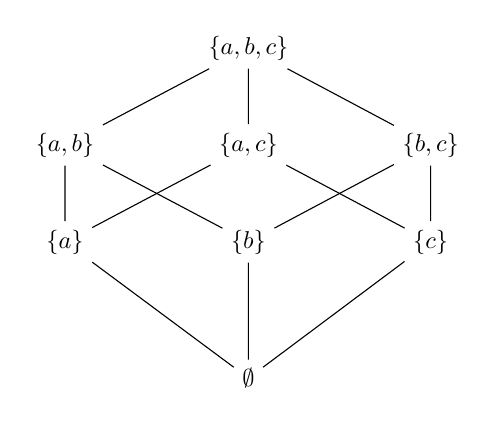
\begin{tikzpicture}[node distance=8mm and 14mm, scale=0.88, transform shape]
    \node (abc) {$\{a,b,c\}$};
    \node[below left=of abc] (ab) {$\{a,b\}$};
    \node[below=of abc] (ac) {$\{a,c\}$};
    \node[below right=of abc] (bc) {$\{b,c\}$};
    \node[below=of ab] (a) {$\{a\}$};
    \node[below=of ac] (b) {$\{b\}$};
    \node[below=of bc] (c) {$\{c\}$};
    \node[below=14mm of b] (e) {$\emptyset$};
    \draw (abc)--(ab) (abc)--(ac) (abc)--(bc);
    \draw (ab)--(a) (ab)--(b);
    \draw (ac)--(a) (ac)--(c);
    \draw (bc)--(b) (bc)--(c);
    \draw (a)--(e) (b)--(e) (c)--(e);
\end{tikzpicture}
\end{center}

Given \(A\subseteq S\), an upper bound \(u\) satisfies \(a\leq u\) for every \(a\in A\), whereas a lower bound \(l\) satisfies \(l\leq a\) for every \(a\in A\).
The least upper bound, when it exists, is the join
\[
    \bigvee A,
\]
while the greatest lower bound is the meet
\[
    \bigwedge A.
\]

\begin{snippetdefinition}{Directed set}
    A non-empty subset \(D\subseteq S\) is \emph{directed} if for every \(x,y\in D\) there exists \(z\in D\) such that
    \[
        x\leq z,
        \qquad
        y\leq z.
    \]
\end{snippetdefinition}

A poset is a \emph{lattice} if every pair has a join and a meet.
It is a \emph{complete lattice} if every subset has a join and a meet.
It is a \emph{dcpo} if every directed subset has a join.
Every complete lattice has
\[
    \bot=\bigvee\emptyset,
    \qquad
    \top=\bigwedge\emptyset.
\]

\subsection{Monotone and Scott-continuous functions}

\begin{snippetdefinition}{Monotonicity}
    Let \((S,\leq_S)\) and \((T,\leq_T)\) be posets.
    A function \(f\colon S\fromto T\) is monotone if
    \[
        x\leq_S y
        \implies
        f(x)\leq_T f(y).
    \]
\end{snippetdefinition}

\begin{snippetdefinition}{Scott continuity}
    Let \(S,T\) be dcpos.
    A monotone function \(f\colon S\fromto T\) is Scott-continuous if for every directed set \(D\subseteq S\)
    \[
        f\left(\bigvee D\right)
        =
        \bigvee f(D).
    \]
\end{snippetdefinition}

\begin{snippetproposition}{}
    Every Scott-continuous function is monotone.
\end{snippetproposition}

\begin{snippetproof}{}
    If \(a\leq b\), then \(\{a,b\}\) is directed and \(\bigvee\{a,b\}=b\).
    Therefore
    \[
        f(b)
        =f(\bigvee\{a,b\})
        =\bigvee\{f(a),f(b)\},
    \]
    hence \(f(a)\leq f(b)\).
\end{snippetproof}

\begin{snippetexercise}{}
    Show that the converse is false: a monotone function need not be Scott-continuous.
\end{snippetexercise}

\subsection{Fixed points}

\begin{snippetdefinition}{Pre-fixed, post-fixed and fixed points}
    Let \(f\colon L\fromto L\). An element \(x\in L\) is
    \begin{enumerate}
        \item a \emph{pre-fixed point} if \(f(x)\leq x\);
        \item a \emph{post-fixed point} if \(x\leq f(x)\);
        \item a \emph{fixed point} if \(f(x)=x\).
    \end{enumerate}
\end{snippetdefinition}

\begin{snippettheorem}{Knaster--Tarski}
    Let \(L\) be a complete lattice and \(f\colon L\fromto L\) monotone.
    Then the set of fixed points of \(f\) is a complete lattice. Moreover,
    \[
        \gfp(f)
        =
        \bigvee\{x\in L\suchthat x\leq f(x)\},
    \]
    and
    \[
        \lfp(f)
        =
        \bigwedge\{x\in L\suchthat f(x)\leq x\}.
    \]
\end{snippettheorem}

\begin{snippetproof}{Construction of the greatest fixed point}
    Put
    \[
        g=\bigvee\{x\suchthat x\leq f(x)\}.
    \]
    For every post-fixed point \(x\), we have \(x\leq g\), hence by monotonicity
    \[
        f(x)\leq f(g).
    \]
    Since \(x\leq f(x)\), we obtain \(x\leq f(g)\) for every post-fixed point, and therefore
    \[
        g\leq f(g).
    \]
    Applying monotonicity again,
    \[
        f(g)\leq f(f(g)),
    \]
    so \(f(g)\) is itself post-fixed. By the definition of \(g\), \(f(g)\leq g\).
    Thus \(f(g)=g\).
    The least fixed point case is dual.
\end{snippetproof}

\begin{snippettheorem}{Kleene fixed-point theorem}
    Let \(L\) be a dcpo with bottom \(\bot\), and let \(f\colon L\fromto L\) be Scott-continuous.
    Then
    \[
        \lfp(f)
        =
        \bigvee_{n\geq0}f^n(\bot).
    \]
\end{snippettheorem}

\begin{snippetproof}{}
    The chain
    \[
        \bot\leq f(\bot)\leq f^2(\bot)\leq\cdots
    \]
    is increasing by monotonicity.
    Put \(p=\bigvee_n f^n(\bot)\). By continuity,
    \[
        f(p)
        =
        f\left(\bigvee_n f^n(\bot)\right)
        =
        \bigvee_n f^{n+1}(\bot)
        =p.
    \]
    If \(q\) is another fixed point, then by induction
    \[
        f^n(\bot)\leq q
    \]
    for every \(n\), hence \(p\leq q\).
\end{snippetproof}

\section{Denotational semantics}

\subsection{Motivations}

Denotational semantics associates a mathematical object with every programming-language construct.
Its two central contributions are \emph{compositionality} and a mathematical characterization of recursion through fixed points.
The main ingredients are therefore functions, complete partial orders, and fixed-point theory.

\subsection{A review of the \(\lambda\)-calculus}

The \(\lambda\)-calculus is a minimal formal language for defining functions, function composition, and function evaluation.
Its syntax is generated by variables, abstractions, and applications:
\[
    e ::= x\mid\lambda x.e\mid e_1e_2.
\]
We parenthesize compound applications explicitly whenever their association matters.

The fundamental computation rule is \(\beta\)-reduction
\[
    (\lambda x.d)e
    \longrightarrow
    d\{e/x\},
\]
where substitution must avoid variable capture.

\begin{snippetexample}{Simple \(\lambda\)-terms}
    \[
        \lambda x.x,
        \qquad
        \lambda x.xx,
        \qquad
        \lambda x.xz,
        \qquad
        \lambda x.kz.
    \]
    We can also use mixed notation such as \(\lambda x.x+1\) when arithmetic operators are already available in the metalanguage.
\end{snippetexample}

Church numerals are
\[
    0\triangleq\lambda f.\lambda x.x,
    \qquad
    1\triangleq\lambda f.\lambda x.fx,
    \qquad
    2\triangleq\lambda f.\lambda x.f(fx),
\]
and in general the numeral \(n\) applies \(f\) exactly \(n\) times.
We can define
\[
    \mathsf{succ}
    \triangleq
    \lambda n.\lambda f.\lambda x.f(nfx),
\]
and, for instance,
\[
    \mathsf{plus}
    \triangleq
    \lambda m.\lambda n.\lambda f.\lambda x.mf(nfx),
\]
or equivalently define addition in terms of \(\mathsf{succ}\).
Then
\[
    \mathsf{succ}\ 2\longrightarrow^*3,
    \qquad
    \mathsf{plus}\ 1\ 2\longrightarrow^*3,
    \qquad
    \mathsf{plus}\ 4\ 2\longrightarrow^*6.
\]

Booleans can also be encoded:
\[
    \mathsf{true}=\lambda x.\lambda y.x,
    \qquad
    \mathsf{false}=\lambda x.\lambda y.y.
\]
Moreover,
\begin{align*}
    \mathsf{and}&\triangleq\lambda p.\lambda q.p\,q\,p,\\
    \mathsf{or}&\triangleq\lambda p.\lambda q.p\,p\,q,\\
    \mathsf{not}&\triangleq\lambda p.\lambda a.\lambda b.p\,b\,a,\\
    \mathsf{cond}&\triangleq\lambda p.\lambda a.\lambda b.p\,a\,b.
\end{align*}
If \(e\longrightarrow^*\mathsf{true}\), then
\[
    \mathsf{cond}\ e\ y\ z\longrightarrow^*y,
\]
and if \(e\longrightarrow^*\mathsf{false}\), the result is \(z\).

Mixed notation emphasizes that ordinary functions can be represented in the same formalism:
\[
    \mathsf{succ}=\lambda x.x+1,
    \qquad
    \mathsf{poly}=\lambda x.x^2-3x+1,
\]
\[
    g=\lambda x.\lambda y.x-y,
    \qquad
    h=\lambda y.\lambda x.x-y.
\]
For instance, \(g\,3\,4\) returns \(3-4\), while \(h\,3\,4\) returns \(4-3\).
The main idea is that all objects of the \(\lambda\)-calculus are represented functionally: numbers, Booleans, states, arithmetic functions, and predicates can all be described in one formalism.

Self-application shows that evaluation need not terminate. Terms such as
\[
    (\lambda x.xx)(\lambda x.xx)
\]
reduce to themselves.
This possibility is essential for representing recursion and divergence.

\subsection{Compositionality for While}

The arithmetic and Boolean semantics defined earlier are already denotational.
For statements we seek a function
\[
    \mathcal S_{ds}\colon\Stm\fromto(\State\not\to\State).
\]

For assignment and skip, define
\[
    \mathcal S_{ds}\sem{x:=a}s
    =s[x\mapsto\mathcal A\sem{a}s],
    \qquad
    \mathcal S_{ds}\sem{\skipc}=\Id.
\]
Sequential composition becomes function composition:
\[
    \mathcal S_{ds}\sem{S_1;S_2}
    =
    \mathcal S_{ds}\sem{S_2}\circ\mathcal S_{ds}\sem{S_1}.
\]
The conditional is
\[
    \mathcal S_{ds}\sem{\mathsf{if}\ b\ \mathsf{then}\ S_1\ \mathsf{else}\ S_2}
    =
    \lambda s.\cond\bigl(
        \mathcal B\sem{b}s,
        \mathcal S_{ds}\sem{S_1}s,
        \mathcal S_{ds}\sem{S_2}s
    \bigr).
\]

\subsection{The while construct as a fixed point}

Let
\[
    W\triangleq\mathsf{while}\ b\ \mathsf{do}\ S.
\]
Its semantics must satisfy
\[
    \mathcal S_{ds}\sem{W}
    =
    F_{b,S}(\mathcal S_{ds}\sem{W}),
\]
where
\[
    F_{b,S}(w)
    =
    \lambda s.\cond\left(
        \mathcal B\sem{b}s,
        w(\mathcal S_{ds}\sem{S}s),
        s
    \right).
\]
Thus we want to define
\[
    \mathcal S_{ds}\sem{W}
    =
    \fix(F_{b,S}),
\]
but we still have to determine which fixed point must be chosen.

\begin{snippetexample}{A recursive equation can have several solutions}
    A definition such as
    \[
        f(x)=
        \begin{cases}
            1 & x=0,\\
            f(x+1) & x\neq0
        \end{cases}
    \]
    does not determine a unique total function.
    Besides the least-defined solution, which returns \(1\) at \(0\) and is undefined elsewhere, there are solutions assigning an arbitrary constant value to points that never reach \(0\).
    Program semantics should select the solution containing only the information forced by the recursive definition.
\end{snippetexample}

\subsection{Information order on partial functions}

For partial functions \(f,g\colon X\not\to Y\), define
\[
    f\sqsubseteq g
    \iff
    \forall x\in X,
    \quad
    f(x)\text{ defined}
    \implies
    f(x)=g(x).
\]
Thus \(g\) contains at least as much information as \(f\).
The everywhere undefined function \(\Omega\) is the bottom element.

For a recursive function we obtain the approximations
\[
    \Omega
    \sqsubseteq
    F(\Omega)
    \sqsubseteq
    F^2(\Omega)
    \sqsubseteq
    \cdots.
\]
For factorial, the successive approximations define the result for progressively more inputs.

\begin{snippetexample}{Approximations of the factorial while loop}
    If the body multiplies an accumulator \(y\) by \(x\) and decrements \(x\), then the limit of the approximation chain is the function
    \[
        f^\omega(x,y)
        =
        \begin{cases}
            (x,y) & x\leq0,\\
            (0,x!\,y) & x\geq1.
        \end{cases}
    \]
    This is the least fixed point of the functional associated with the loop.
\end{snippetexample}

\subsection{CPOs and the fixed-point theorem}

A CPO is a poset with bottom in which every increasing chain has a least upper bound.
The set of partial functions ordered by information is a CPO.

The semantic functions used here are monotone and continuous with respect to this order, and composition preserves continuity.
By Kleene's theorem,
\[
    \fix(F)
    =
    \lfp(F)
    =
    \bigvee_{n\geq0}F^n(\bot).
\]

This makes the semantics of while well defined: the domain of state functions is a CPO, the conditional is continuous, composition preserves continuity, and the loop functional is continuous.

\begin{snippettheorem}{Equivalence of SOS and denotational semantics}
    For every statement \(S\),
    \[
        \mathcal S_{sos}\sem{S}
        =
        \mathcal S_{ds}\sem{S}.
    \]
\end{snippettheorem}

The proof uses a stronger invariant for a single SOS step and proceeds first by structural induction on the constructs and then by induction on the length of computations.

\pagebreak
\part{Induction and coinduction}

\section{Examples of induction and coinduction}

Induction and coinduction are dual principles.
Induction describes objects constructed in finitely many steps and reasons about the \emph{least} set closed under a collection of rules.
Coinduction also describes potentially infinite behaviour and reasons about the \emph{greatest} set compatible with suitable observations.

\subsection{Mathematical induction and a non-example}

Recall the principle of mathematical induction. A variant of the inductive step assumes the property for all natural numbers less than or equal to \(n\).
Other variants are possible, for instance by changing the basis.

\begin{snippetexample}{A false proof by induction}
    Consider the statement ``all men have eyes of the same colour''.
    The case of one man is trivial.
    Assume that every set of \(n\) men has only one eye colour, and consider \(n+1\) ordered men.
    The subsets in positions
    \[
        \{1,\ldots,n\}
        \qquad\text{and}\qquad
        \{2,\ldots,n+1\}
    \]
    both contain \(n\) elements, so by the inductive hypothesis each subset would have a single eye colour.
    The argument then concludes that the two colours coincide because the subsets overlap.

    The mistake occurs in the step from \(n=1\) to \(n=2\): the two subsets are disjoint, so there is no common person forcing the two colours to coincide.
\end{snippetexample}

\subsection{Rule induction: finite traces}

Consider an LTS and say that a process is \emph{stopped} if it cannot perform any transition.
Write
\[
    P\downarrow
\]
if \(P\) has a finite sequence of transitions leading to a stopped process.
This property, also called \emph{may termination}, is inductively defined by
\[
    \frac{P\text{ stopped}}{P\downarrow},
    \qquad
    \frac{P\trans{\mu}P'\qquad P'\downarrow}{P\downarrow}.
\]

A set inductively defined by rules admits three equivalent readings:
\begin{enumerate}
    \item the set of elements having a finite, or more generally well-founded, proof tree;
    \item the least set closed \emph{forwards} under the rules;
    \item the set obtained by an iterative construction starting from the empty set.
\end{enumerate}
We will justify all three readings through fixed-point theory.

\begin{snippetdefinition}{Forward closure}
    A set \(T\) is closed forwards under a system of rules if, whenever all premises of a rule belong to \(T\), its conclusion also belongs to \(T\).
\end{snippetdefinition}

For \(\downarrow\), every forward-closed set must contain all stopped processes and, whenever it contains a derivative \(P'\) reachable from \(P\), it must also contain \(P\).
The least set with this property is exactly the set of processes having a finite trace to a stopped state.

\begin{snippetexample}{A function defined on terminating processes}
    Define partially
    \[
        f(P)=\text{minimum length of a trace from \(P\) to a stopped process}.
    \]
    The domain of \(f\) is closed forwards under the rules for \(\downarrow\): stopped processes are in the domain and, if \(P\trans{\mu}P'\) with \(P'\in\dom(f)\), then \(P\in\dom(f)\) as well.
    By rule induction,
    \[
        \{P\suchthat P\downarrow\}\subseteq\dom(f).
    \]
\end{snippetexample}

\subsection{Rule coinduction: infinite traces}

Write
\[
    P\uparrow
\]
if \(P\) can perform an infinite trace.
The coinductive definition uses only the rule
\[
    \frac{P\trans{\mu}P'\qquad P'\uparrow}{P\uparrow}.
\]
There is no base case: a proof may be infinite.

The dual coinductive reading is:
\begin{enumerate}
    \item proof trees need not be well founded;
    \item we look for the greatest set closed \emph{backwards};
    \item we start from the universe of all processes and progressively remove those that cannot satisfy the rule.
\end{enumerate}

\begin{snippetdefinition}{Backward closure}
    A set \(T\) is closed backwards under the rules if, for every \(x\in T\), there exists at least one rule with conclusion \(x\) whose premises all belong to \(T\).
\end{snippetdefinition}

Thus, to prove \(P\uparrow\), we do not necessarily have to construct the whole infinite trace.
It is enough to find a candidate set \(T\) containing \(P\) such that every process in \(T\) has at least one transition to another element of \(T\).

\begin{snippetexample}{Coinductive proof of divergence}
    If \(P_1\trans{a}P_2\) and \(P_2\trans{b}P_1\), take
    \[
        T=\{P_1,P_2\}.
    \]
    Every element of \(T\) has a transition to another element of \(T\), so \(T\) is backward closed and
    \[
        P_1\uparrow,
        \qquad
        P_2\uparrow.
    \]
\end{snippetexample}

\subsection{Finite and infinite lists}

Fix a set \(A\). Finite lists are inductively defined by
\[
    \frac{}{\nil\in\mathsf{finLists}},
    \qquad
    \frac{\ell\in\mathsf{finLists}\qquad a\in A}
    {\langle a\rangle\cdot\ell\in\mathsf{finLists}}.
\]

If the same observation pattern is interpreted coinductively, we obtain both finite and infinite lists.
A coinductive object is observed through destructors: a list is \(\nil\), or it exposes a head \(a\) and a tail that is again a list.

\subsection{Convergence and divergence in the \(\lambda\)-calculus}

Under call-by-name, convergence \(e\Downarrow e'\) can be inductively defined by
\[
    \frac{}{\lambda x.e\Downarrow\lambda x.e},
\]
\[
    \frac{
        e_1\Downarrow\lambda x.e_0
        \qquad
        e_0\{e_2/x\}\Downarrow e'
    }{
        e_1e_2\Downarrow e'
    }.
\]

Divergence \(e\Uparrow\) is instead coinductive:
\[
    \frac{e_1\Uparrow}{e_1e_2\Uparrow},
    \qquad
    \frac{
        e_1\Downarrow\lambda x.e_0
        \qquad
        e_0\{e_2/x\}\Uparrow
    }{
        e_1e_2\Uparrow}.
\]
The first system describes the least convergence relation compatible with the rules, whereas the second describes the greatest set of terms compatible with the observations of divergence.

\section{Duality between induction and coinduction}

Induction is driven by \emph{constructors}: to belong to an inductively defined set, an object must be obtained from base cases by finitely many applications of the constructors.
Coinduction is driven by \emph{observers}: an object belongs to a coinductively defined set when it keeps producing admissible observations.

The main correspondences are:
\begin{center}
\begin{tabular}{c|c}
Induction & Coinduction \\
\hline
least set & greatest set \\
forward closure & backward closure \\
least fixed point & greatest fixed point \\
pre-fixed points & post-fixed points \\
constructors & observers/destructors \\
congruences & bisimulations \\
substitutive relations & bisimulative relations \\
identity/syntax & bisimilarity/semantics \\
algebras & coalgebras \\
well-founded proofs & possibly non-well-founded proofs \\
strengthen the candidate & weaken/enlarge the candidate
\end{tabular}
\end{center}

For instance, a congruence is typically defined forwards: if two components are related, applying a constructor produces related objects again.
A bisimulation is instead defined backwards from observations: every observation on one side must be matched by the other side.

The two techniques interact in process algebra: we want bisimilarity, obtained coinductively, to be a congruence with respect to the syntactic operators.

\section{Fixed-point theory for induction and coinduction}

\subsection{Complete lattices}

Consider a complete lattice \((L,\leq)\).
Every set \(S\subseteq L\) has both a meet and a join.
For the fundamental example \(L=\powerset(X)\), the order is inclusion and
\[
    \bigvee_i S_i = \bigcup_i S_i,
    \qquad
    \bigwedge_i S_i = \bigcap_i S_i,
    \qquad
    \bot=\emptyset,
    \qquad
    \top=X.
\]

\begin{snippetexample}{Divisibility order}
    Consider the positive natural numbers ordered by
    \[
        n\leq m
        \iff
        n\mid m.
    \]
    For \(S=\{4,8,16\}\), the lower bounds are \(\{1,2,4\}\), the meet is \(4\), and \(16\) is both the maximum and the join.
    For \(S=\{2,3,4\}\), the meet is \(1\), there is no minimum element of \(S\), the upper bounds are the multiples of \(12\), the join is \(12\), and there is no maximum.
\end{snippetexample}

\begin{snippetexample}{Pre-fixed points and fixed points}
    On the positive natural numbers, let \(F(n)\) be the sum of the proper divisors of \(n\), with the exception \(F(1)=1\).
    For example,
    \[
        F(1)=1,
        \quad
        F(2)=1,
        \quad
        F(3)=1,
        \quad
        F(4)=3,
        \quad
        F(6)=6.
    \]
    With respect to divisibility, \(1,2,3,6\) are pre-fixed points and \(1,6\) are fixed points.
\end{snippetexample}

\begin{snippetexercise}{}
    Determine whether \(\naturalnumbers\) is a complete lattice and whether it is at least a lattice.
    Determine also which elements can be added to obtain a complete lattice.
\end{snippetexercise}

\begin{snippetexercise}{}
    Let \(F\) be monotone on a complete lattice.
    Show that the join of two post-fixed points is again post-fixed, generalize to an arbitrary family, and give the dual result for pre-fixed points.
\end{snippetexercise}

\subsection{Fixed-point theorem}

For simplicity, first state the theorem on \(\powerset(X)\).

\begin{snippettheorem}{Fixed-point theorem}
    Let
    \[
        F\colon\powerset(X)\fromto\powerset(X)
    \]
    be monotone. Then
    \[
        \lfp(F)
        =
        \bigcap\{T\subseteq X\suchthat F(T)\subseteq T\},
    \]
    and
    \[
        \gfp(F)
        =
        \bigcup\{T\subseteq X\suchthat T\subseteq F(T)\}.
    \]
    Thus the least fixed point is the meet of all pre-fixed points and the greatest fixed point is the join of all post-fixed points.
\end{snippettheorem}

The fixed points, pre-fixed points, and post-fixed points themselves inherit complete-lattice structure.

\begin{snippetproof}{Greatest fixed point}
    Put
    \[
        T=\bigcup\{S\subseteq X\suchthat S\subseteq F(S)\}.
    \]
    For every post-fixed point \(S\), \(S\subseteq T\), hence by monotonicity
    \[
        F(S)\subseteq F(T).
    \]
    Since \(S\subseteq F(S)\), we obtain \(S\subseteq F(T)\).
    Taking the union over all post-fixed points gives
    \[
        T\subseteq F(T).
    \]
    Applying \(F\) and monotonicity,
    \[
        F(T)\subseteq F(F(T)),
    \]
    so \(F(T)\) is post-fixed.
    Since \(T\) is the union of all post-fixed points,
    \[
        F(T)\subseteq T.
    \]
    Therefore \(F(T)=T\), and \(T\) is the greatest fixed point.
\end{snippetproof}

\begin{snippetdefinition}{Inductive and coinductive sets of a functional}
    Given a monotone endofunctional \(F\) on a complete lattice of sets, define
    \[
        F_{\mathrm{ind}}
        \triangleq
        \lfp(F),
        \qquad
        F_{\mathrm{coind}}
        \triangleq
        \gfp(F).
    \]
\end{snippetdefinition}

\subsection{From rules to functionals}

\begin{snippetdefinition}{Ground rule}
    Let \(X\) be a set.
    A ground rule over \(X\) is a pair
    \[
        (S,x),
        \qquad
        S\subseteq X,
        \quad
        x\in X.
    \]
    We write it as
    \[
        \frac{x_1\quad x_2\quad\cdots}{x},
        \qquad
        S=\{x_1,x_2,\ldots\}.
    \]
    A rule \((\emptyset,x)\) is an axiom.
\end{snippetdefinition}

Rules with meta-variables are not ground, but they can be translated into ground rules by taking all valid instantiations.

\begin{snippetdefinition}{Functional associated with a rule system}
    Given a set of ground rules \(R\) over \(X\), define
    \[
        \Phi_R(T)
        \triangleq
        \{x\in X\suchthat
        \exists (S,x)\in R,\ S\subseteq T\}.
    \]
\end{snippetdefinition}

\begin{snippetproposition}{}
    \(\Phi_R\) is monotone.
\end{snippetproposition}

\begin{snippetexercise}{}
    Show that every monotone operator on \(\powerset(X)\) can be represented as the functional associated with a suitable set of ground rules.
\end{snippetexercise}

By the fixed-point theorem,
\[
    \lfp(\Phi_R)
\]
is the set inductively defined by the rules, while
\[
    \gfp(\Phi_R)
\]
is the set coinductively defined by them.

The condition
\[
    \Phi_R(T)\subseteq T
\]
says exactly that \(T\) is forward closed: every axiom concludes an element of \(T\), and every rule whose premises are in \(T\) has its conclusion in \(T\).
Thus rule induction is the principle
\[
    \Phi_R(T)\subseteq T
    \implies
    \lfp(\Phi_R)\subseteq T.
\]

Dually,
\[
    T\subseteq\Phi_R(T)
\]
says that \(T\) is backward closed, and rule coinduction is
\[
    T\subseteq\Phi_R(T)
    \implies
    T\subseteq\gfp(\Phi_R).
\]

\begin{snippetexercise}{}
    Suppose every rule in \(R\) has a non-empty set of premises.
    Show that
    \[
        \lfp(\Phi_R)=\emptyset.
    \]
\end{snippetexercise}

\subsection{Examples in fixed-point form}

For finite traces, the ground rules are
\[
    R_\downarrow
    =
    \{(\emptyset,P)\suchthat P\text{ stopped}\}
    \union
    \{(\{P'\},P)\suchthat P\trans{\mu}P'\text{ for some }\mu\}.
\]
Therefore
\[
    \Phi_{R_\downarrow}(T)
    =
    \{P\suchthat P\text{ is stopped, or }P\trans{\mu}P'\text{ with }P'\in T\}.
\]
The processes having a finite trace form \(\lfp(\Phi_{R_\downarrow})\).

For infinite traces,
\[
    R_\uparrow
    =
    \{(\{P'\},P)\suchthat P\trans{\mu}P'\},
\]
and
\[
    \Phi_{R_\uparrow}(T)
    =
    \{P\suchthat \exists P'\in T,\ P\trans{\mu}P'\}.
\]
The processes having an infinite trace form \(\gfp(\Phi_{R_\uparrow})\).

For finite lists,
\[
    F(T)
    =
    \{\nil\}
    \union
    \{\langle a\rangle\cdot\ell\suchthat a\in A,\ \ell\in T\}.
\]
Hence
\[
    \mathsf{finLists}=\lfp(F).
\]
List induction is precisely the pre-fixed-point principle applied to this functional.

For the \(\lambda\)-calculus, the convergence functional acts on relations of pairs of closed terms:
\begin{align*}
    \Phi_\Downarrow(T)
    ={}&
    \{(e,e')\suchthat e=e'=\lambda x.e''\text{ for some }e''\}\\
    &\union
    \{(e,e')\suchthat e=e_1e_2,\
    \exists e_0:\ (e_1,\lambda x.e_0)\in T,
    (e_0\{e_2/x\},e')\in T\}.
\end{align*}
For divergence,
\[
    \Phi_\Uparrow(T)
    =
    \{e_1e_2\suchthat e_1\in T\}
    \union
    \{e_1e_2\suchthat e_1\Downarrow\lambda x.e_0,\ e_0\{e_2/x\}\in T\}.
\]

\subsection{Bisimulation on lists}

Coinduction is not specific to concurrency.
Consider finite or infinite lists and the LTS
\[
    \langle a\rangle\cdot s\trans{a}s.
\]

\begin{snippetdefinition}{List bisimulation}
    A relation \(R\) on lists is a list bisimulation if, for every \((s,t)\in R\),
    \begin{enumerate}
        \item \(s=\nil\implies t=\nil\);
        \item if \(s=\langle a\rangle\cdot s'\), then there exists \(t'\) such that
        \[
            t=\langle a\rangle\cdot t'
            \qquad\text{and}\qquad
            (s',t')\in R.
        \]
    \end{enumerate}
    List bisimilarity is the union of all list bisimulations.
\end{snippetdefinition}

\begin{snippetproposition}{}
    For finite or infinite lists,
    \[
        s=t
        \iff
        s\sim t.
    \]
\end{snippetproposition}

Equality itself can be presented coinductively by the rules
\[
    \frac{}{\nil=\nil},
    \qquad
    \frac{s_1=s_2\qquad a\in A}
    {\langle a\rangle\cdot s_1=\langle a\rangle\cdot s_2}.
\]
The inductive interpretation gives equality on finite lists; the coinductive interpretation also includes infinite lists, and its post-fixed points are precisely the list bisimulations.

\begin{snippetexample}{Coinduction with \(\mathsf{map}\) and \(\mathsf{iterate}\)}
    Let \(f\colon A\fromto A\) and define
    \begin{align*}
        \mathsf{map}\ f\ \nil &= \nil,\\
        \mathsf{map}\ f\ (\langle a\rangle\cdot s)
        &=\langle f(a)\rangle\cdot\mathsf{map}\ f\ s,\\
        \mathsf{iterate}\ f\ a
        &=\langle a\rangle\cdot\mathsf{iterate}\ f\ f(a).
    \end{align*}
    We want to prove
    \[
        \mathsf{map}\ f\ (\mathsf{iterate}\ f\ a)
        =
        \mathsf{iterate}\ f\ f(a).
    \]
    Take
    \[
        R
        =
        \{(
        \mathsf{map}\ f\ (\mathsf{iterate}\ f\ a),
        \mathsf{iterate}\ f\ f(a))
        \suchthat a\in A\}.
    \]
    Both sides expose the head \(f(a)\), and the resulting tails are again related by \(R\).
    Thus \(R\) is a bisimulation and the result follows by coinduction.
\end{snippetexample}

\section{Other induction and coinduction principles}

\subsection{Mathematical induction as rule induction}

The rules
\[
    \frac{}{0},
    \qquad
    \frac{n}{n+1}
    \quad(n\geq0)
\]
inductively define the natural numbers.
Thus rule induction coincides with mathematical induction.

The strong variant uses rules of the form
\[
    \frac{0,1,\ldots,n}{n+1},
\]
or, in open form,
\[
    \frac{i\in S\text{ for every }i<j}{j\in S}.
\]

\subsection{Well-founded induction}

\begin{snippettheorem}{Well-founded induction}
    Let \(R\) be a well-founded relation on \(X\).
    To prove a property \(T\) for all elements of \(X\), it is enough to prove for every \(x\in X\) that
    \[
        \left(\forall y,\ yRx\implies y\in T\right)
        \implies
        x\in T.
    \]
\end{snippettheorem}

Mathematical induction and structural induction are special cases.
A common example is induction on the lexicographic order of pairs of natural numbers.

The principle can be derived from rule induction by choosing, for every \(x\), the rule
\[
    \frac{\{y\suchthat yRx\}}{x}.
\]
If \(R\) is well founded, the inductively generated set is all of \(X\).

\subsection{Transfinite induction}

Transfinite induction extends mathematical induction to ordinals.
To prove a property \(T\) for all ordinals, show that
\[
    \left(\forall\beta<\alpha,\ \beta\in T\right)
    \implies
    \alpha\in T.
\]
In practice, one distinguishes three cases:
\begin{enumerate}
    \item \(0\in T\);
    \item if \(\alpha\in T\), then \(\alpha+1\in T\);
    \item if \(\beta\) is a limit ordinal and \(\alpha\in T\) for every \(\alpha<\beta\), then \(\beta\in T\).
\end{enumerate}

The ordinals form a proper class, so this formulation is not obtained directly from the set-based lattice theory developed here.
In applications, however, ordinals can be used to rank elements of a set, inducing a well-founded relation; transfinite induction then becomes an instance of well-founded induction.

Other common induction principles include structural induction, induction on derivation trees, and induction on transitions.

\subsection{Recursion and corecursion}

A function defined by \emph{recursion} typically has an inductive domain.
Examples are
\[
    f(0)=1,
    \qquad
    f(n+1)=n\,f(n),
\]
and structural recursion on \(\lambda\)-terms
\begin{align*}
    f(x)&=0,\\
    f(\lambda x.e)&=1+f(e),\\
    f(ee')&=f(e)+f(e').
\end{align*}
General schemes of well-founded recursion exist; well-founded induction can be used to prove existence and uniqueness of the specified function.

A function defined by \emph{corecursion} instead produces an element of a coinductive set.
The equations specify the immediate observations of the produced object: for an infinite list, for example, they determine the head and how to obtain the tail.
The functions \(\mathsf{map}\) and \(\mathsf{iterate}\) are natural examples.
General corecursion schemes similarly provide existence and uniqueness, including mutually corecursive systems of equations.

\subsection{Coinduction up-to}

The coinduction principle can be strengthened by allowing the candidate to be closed using relations that are already known.

\begin{snippettheorem}{Coinduction up-to join}
    Let \(F\) be monotone on a complete lattice and let \(y\) be a post-fixed point, that is,
    \[
        y\leq F(y).
    \]
    Then
    \[
        \gfp(F)
        =
        \bigvee\{x\suchthat x\leq F(x\vee y)\}.
    \]
    In particular,
    \[
        x\leq F(x\vee y)
        \implies
        x\leq\gfp(F).
    \]
\end{snippettheorem}

A more general principle is coinduction \emph{up-to gfp}.
Let \(\bullet\colon L\cartesianprod L\fromto L\) be associative and assume:
\begin{enumerate}
    \item if \(x\leq F(x')\) and \(y\leq F(y')\), then
    \[
        x\bullet y\leq F(x'\bullet y');
    \]
    \item for every post-fixed point \(x\),
    \[
        x\leq x\bullet\gfp(F),
        \qquad
        x\leq\gfp(F)\bullet x.
    \]
\end{enumerate}
Then
\[
    x\leq F(\gfp(F)\bullet x\bullet\gfp(F))
    \implies
    x\leq\gfp(F).
\]

\section{Bisimilarity as a fixed point}

Let \(\Proc\) be the set of states of an LTS.
Define
\[
    F_{\sim}\colon\powerset(\Proc\cartesianprod\Proc)
    \fromto
    \powerset(\Proc\cartesianprod\Proc)
\]
by putting \((P,Q)\in F_{\sim}(R)\) if, for every action \(\mu\),
\begin{enumerate}
    \item every \(P\trans{\mu}P'\) is matched by some \(Q\trans{\mu}Q'\) with \(P'RQ'\);
    \item symmetrically, every \(Q\trans{\mu}Q'\) is matched by some \(P\trans{\mu}P'\) with \(P'RQ'\).
\end{enumerate}

\begin{snippetproposition}{}
    \begin{enumerate}
        \item \(F_{\sim}\) is monotone;
        \item \(R\) is a bisimulation if and only if
        \[
            R\subseteq F_{\sim}(R);
        \]
        \item bisimilarity is
        \[
            \sim\;=\gfp(F_{\sim}).
        \]
    \end{enumerate}
\end{snippetproposition}

This formulation explains formally why bisimulation is a coinductive proof method.

\section{Constructive approximations of fixed points}

\subsection{Continuity and cocontinuity}

The fixed-point theorem above is existential and does not by itself give an iterative algorithm.
To obtain fixed points constructively, introduce continuity and cocontinuity.

\begin{snippetdefinition}{Continuity and cocontinuity}
    An endofunctional \(F\) on a complete lattice is
    \begin{enumerate}
        \item \emph{continuous} if for every increasing chain \(T_0\leq T_1\leq\cdots\),
        \[
            F\left(\bigvee_iT_i\right)
            =
            \bigvee_iF(T_i);
        \]
        \item \emph{cocontinuous} if for every decreasing chain \(T_0\geq T_1\geq\cdots\),
        \[
            F\left(\bigwedge_iT_i\right)
            =
            \bigwedge_iF(T_i).
        \]
    \end{enumerate}
\end{snippetdefinition}

\begin{snippetexample}{}
    Consider the integers extended with two points \(-\omega\) and \(\omega\), ordered naturally, and define
    \[
        F(n)=n+1,
        \qquad
        F(\omega)=\omega,
        \qquad
        F(-\omega)=-\omega.
    \]
    On increasing chains of positive integers and decreasing chains of negative integers, the operator preserves the relevant joins and meets.
\end{snippetexample}

\begin{snippetexercise}{}
    Show that every continuous or cocontinuous function is monotone.
    For \(x\geq y\), use an eventually constant chain such as \(x,y,y,\ldots\) in the appropriate direction.
\end{snippetexercise}

Define the iterates
\[
    F^0(x)=x,
    \qquad
    F^{n+1}(x)=F(F^n(x)),
\]
and
\[
    F^{\cup\omega}(x)=\bigvee_{n\geq0}F^n(x),
    \qquad
    F^{\cap\omega}(x)=\bigwedge_{n\geq0}F^n(x).
\]

\begin{snippettheorem}{Continuity/Cocontinuity theorem}
    Let \(F\) be an endofunctional on a complete lattice.
    \begin{enumerate}
        \item If \(F\) is continuous,
        \[
            \lfp(F)=F^{\cup\omega}(\bot).
        \]
        \item If \(F\) is cocontinuous,
        \[
            \gfp(F)=F^{\cap\omega}(\top).
        \]
    \end{enumerate}
\end{snippettheorem}

\begin{snippetexercise}{}
    Prove the theorem. For the cocontinuous case, first prove that \(F^{\cap\omega}(\top)\) is a fixed point and then prove that it is the greatest one using the definition of meet.
\end{snippetexercise}

If \(F\) is only monotone, in general we only know
\[
    \gfp(F)\leq F^{\cap\omega}(\top).
\]
Equality may fail.

\begin{snippetexample}{Monotonicity without cocontinuity}
    Consider the order consisting of the negative integers together with \(-\omega\) and \(-(\omega+1)\), ordered so that
    \[
        -n\geq-\omega\geq-(\omega+1).
    \]
    Define
    \[
        F(-n)=-(n+1),
        \qquad
        F(-\omega)=-(\omega+1),
        \qquad
        F(-(\omega+1))=-(\omega+1).
    \]
    Then \(F\) is monotone but not cocontinuous,
    \[
        F^{\cap\omega}(-1)=-\omega,
        \qquad
        \gfp(F)=-(\omega+1).
    \]
\end{snippetexample}

With monotonicity alone, the greatest fixed point can be reached by transfinite iteration:
\begin{align*}
    F^0(\top)&=\top,\\
    F^{\lambda+1}(\top)&=F(F^\lambda(\top)),\\
    F^\lambda(\top)&=\bigwedge_{\beta<\lambda}F^\beta(\top)
    \quad\text{for limit \(\lambda\)}.
\end{align*}
Iterating sufficiently far yields
\[
    F^\infty(\top)=\gfp(F).
\]
The dual result holds for least fixed points.

\subsection{Continuity and cocontinuity of rule systems}

A rule functional need not be continuous.
For example, a rule with infinitely many premises
\[
    \frac{a_1\quad a_2\quad\cdots}{a}
\]
may have its conclusion enabled in the union of a chain without being enabled in any finite element of the chain.

\begin{snippetdefinition}{Finite in the premises}
    A set of rules \(R\) is \emph{FP} if every rule has a finite set of premises.
\end{snippetdefinition}

\begin{snippetproposition}{}
    If \(R\) is FP, then \(\Phi_R\) is continuous. Hence
    \[
        \lfp(\Phi_R)
        =
        \Phi_R^{\cup\omega}(\emptyset).
    \]
\end{snippetproposition}

FP does not imply cocontinuity.
Consider
\[
    X=\{b\}\union\{a_1,a_2,\ldots\}
\]
and one rule \(a_i/b\) for every \(i\).
Then
\[
    \Phi(T)=
    \begin{cases}
        \{b\} & \exists i,\ a_i\in T,\\
        \emptyset & \text{otherwise}.
    \end{cases}
\]
For the decreasing chain
\[
    T_i=\{a_j\suchthat j\geq i\},
\]
we have
\[
    \Phi\left(\bigcap_iT_i\right)=\emptyset,
    \qquad
    \bigcap_i\Phi(T_i)=\{b\}.
\]

\begin{snippetdefinition}{Finite in the conclusions}
    A rule system \(R\) is \emph{FC} if, for every conclusion \(x\), there are only finitely many premise sets \(S\) such that \((S,x)\in R\).
\end{snippetdefinition}

\begin{snippettheorem}{}
    If \(R\) is FC, then \(\Phi_R\) is cocontinuous. Hence
    \[
        \gfp(\Phi_R)
        =
        \Phi_R^{\cap\omega}(X).
    \]
\end{snippettheorem}

Without FC we still have
\[
    \gfp(\Phi_R)
    \subseteq
    \Phi_R^{\cap\omega}(X).
\]

\subsection{Iterative reading of the examples}

For finite traces,
\[
    P\in\Phi_{R_\downarrow}^n(\emptyset)
\]
if and only if there exists a sequence of at most \(n-1\) transitions from \(P\) to a stopped process.
Initially the approximation is empty; then we add stopped processes, then processes having a stopped derivative, and so on.
On a finite LTS the chain stabilizes after finitely many steps.

For infinite traces,
\[
    P\in\Phi_{R_\uparrow}^n(\Proc)
\]
if and only if \(P\) can perform at least \(n\) consecutive transitions.
We start from all processes; at the first step we remove states without derivatives, at the second step those that cannot perform two steps, and so on.
On a finite system this chain also stabilizes after finitely many steps.

\subsection{Approximants of bisimilarity}

Define
\[
    \sim_0 = \Proc\cartesianprod\Proc.
\]
Inductively, \(P\sim_{n+1}Q\) if every transition of \(P\) can be matched by \(Q\) with derivatives in \(\sim_n\), and conversely.
Put
\[
    \sim_\omega
    =
    \bigcap_{n\geq0}\sim_n.
\]
Thus level \(n\) compares behaviours only up to depth \(n\).

\begin{snippetproposition}{}
    The sequence
    \[
        \sim_0\supseteq\sim_1\supseteq\sim_2\supseteq\cdots
    \]
    is decreasing and
    \[
        \sim_n
        =
        F_{\sim}^n(\Proc\cartesianprod\Proc),
        \qquad
        \sim_\omega
        =
        F_{\sim}^{\cap\omega}(\Proc\cartesianprod\Proc).
    \]
\end{snippetproposition}

Approximants are also useful to prove non-bisimilarity: it is enough to find a finite depth at which the pair is removed.

\begin{snippetexample}{\(\sim_\omega\) can be larger than \(\sim\)}
    Consider states \(a_0,a_1,\ldots,a_\omega\) with
    \[
        a_0=0,
        \qquad
        a_n\trans{a}a_{n-1}\quad(n\geq1),
        \qquad
        a_\omega\trans{a}a_\omega.
    \]
    Let \(P\) have an \(a\)-transition to every \(a_n\), \(n\geq0\), and let \(Q\) have the same transitions plus
    \[
        Q\trans{a}a_\omega.
    \]
    For every finite depth \(n\), \(P\sim_nQ\), hence \(P\sim_\omega Q\).
    However, \(P\not\sim Q\): the transition of \(Q\) to \(a_\omega\) can only be matched by \(P\) by choosing some finite \(a_n\), which eventually stops and is not bisimilar to \(a_\omega\).
    Thus \(F_{\sim}\) is not cocontinuous in general.
\end{snippetexample}

\begin{snippetdefinition}{Finite branching}
    An LTS is \emph{finitely branching} if every process has finitely many immediate derivatives.
\end{snippetdefinition}

\begin{snippettheorem}{}
    On finitely branching LTSs,
    \[
        \sim\;=\sim_\omega.
    \]
\end{snippettheorem}

\begin{snippetproof}{}
    The inclusion \(\sim\subseteq\sim_\omega\) follows by showing \(\sim\subseteq\sim_n\) for every \(n\).
    Conversely, put
    \[
        R=\{(P,Q)\suchthat P\sim_\omega Q\}.
    \]
    Let \((P,Q)\in R\) and \(P\trans{\mu}P'\).
    For every \(n\), from \(P\sim_{n+1}Q\) there exists
    \[
        Q\trans{\mu}Q_n
        \qquad\text{with}\qquad
        P'\sim_nQ_n.
    \]
    By finite branching, there are only finitely many possible \(Q_n\), so one derivative \(Q_i\) occurs for infinitely many values of \(n\).
    Since the approximants are decreasing,
    \[
        P'\sim_nQ_i
        \qquad\forall n,
    \]
    and therefore \(P'\sim_\omega Q_i\).
    The symmetric case is analogous, so \(R\) is a bisimulation.
\end{snippetproof}

\subsection{Algorithms for bisimilarity}

The approximant iteration underlies algorithms for checking bisimilarity and minimizing the state space of finite-state processes.
The basic idea is partition refinement: initially all states are in one block, then states that cannot match one another are progressively separated.

The relevant complexity results are:
\begin{itemize}
    \item the bisimulation problem is P-complete;
    \item for a system with \(m\) transitions and \(n\) states there are algorithms running in
    \[
        O(m\log n)
    \]
    time and \(O(m+n)\) space, such as the Paige--Tarjan algorithm;
    \item trace equivalence and testing equivalence are PSPACE-complete.
\end{itemize}

\section{Interpretation by proof trees}

\begin{snippetdefinition}{Proof tree}
    Let \(R\) be a set of ground rules over \(X\).
    An \(X\)-labelled tree is a \emph{proof tree} for \(x\) if the root is labelled \(x\) and, for every node labelled \(y\), if \(S\) is the set of labels of its children, then
    \[
        (S,y)\in R.
    \]
\end{snippetdefinition}

Proof trees may be infinite in depth or width; children of the same node are assumed to carry distinct labels.
A tree is well founded if it contains no infinite path.

For lists, a finite proof builds a finite list.
A periodic infinite list instead gives an infinite proof tree: it is valid coinductively but not inductively.

\begin{snippettheorem}{}
    \[
        x\in\lfp(\Phi_R)
        \iff
        \text{there exists a well-founded proof tree for \(x\)}.
    \]
\end{snippettheorem}

The result can be proved through approximants.
If \(R\) is FP, every node has finitely many children and a well-founded proof tree has finite height; in the examples of traces, lists, and the \(\lambda\)-calculus, inductive objects therefore admit finite derivations.
Without FP, a well-founded tree need not have finite height.

\begin{snippettheorem}{}
    \[
        x\in\gfp(\Phi_R)
        \iff
        \text{there exists a proof tree, possibly non-well-founded, for \(x\)}.
    \]
\end{snippettheorem}

\begin{snippetproof}{}
    If \(x\in\gfp(\Phi_R)\), then there exists a post-fixed point \(T\) with \(x\in T\).
    For every \(y\in T\), choose a rule
    \[
        (S_y,y)\in R,
        \qquad
        S_y\subseteq T.
    \]
    Build the tree starting from \(x\) and using \(S_y\) as the set of children of every node labelled \(y\).

    Conversely, given a proof tree for \(x\), let \(T\) be the set of all node labels.
    For every \(y\in T\), the children of the corresponding node form a set \(S\subseteq T\) with \((S,y)\in R\), hence
    \[
        y\in\Phi_R(T).
    \]
    Therefore \(T\subseteq\Phi_R(T)\), so \(T\) is post-fixed and \(x\in\gfp(\Phi_R)\).
\end{snippetproof}

\section{Interpretation by games}

Another reading of induction and coinduction uses a game between two players:
\begin{itemize}
    \item the \emph{verifier} \(V\), who tries to construct a proof tree;
    \item the \emph{refuter} \(R\), who tries to challenge the derivation.
\end{itemize}

Given \(x_0\in X\), a play has the form
\[
    x_0,S_0,x_1,S_1,\ldots.
\]
The verifier chooses \(S_i\) such that \((S_i,x_i)\in R\), that is, a rule with conclusion \(x_i\).
The refuter then chooses an element \(x_{i+1}\in S_i\), challenging the verifier to justify that premise.

A play ends when one of the players cannot move, and that player loses.
If the play is infinite, the convention depends on the interpretation:
\begin{enumerate}
    \item in the inductive game the refuter wins, because proofs must be well founded;
    \item in the coinductive game the verifier wins, because infinite derivations are allowed.
\end{enumerate}

\begin{snippetexample}{Game for divergence in the \(\lambda\)-calculus}
    Let
    \[
        e_1=\lambda x.xx.
    \]
    For \(e_1e_1\), the verifier can produce the infinite play
    \[
        e_1e_1,\{e_1e_1\},e_1e_1,\ldots,
    \]
    which is winning in the coinductive game.

    For \(e_2=\lambda x.xxx\), an infinite play winning for \(V\) exists as well, while a bad choice may lead to a finite play won by the refuter.
\end{snippetexample}

\begin{snippetexample}{Game for finite traces}
    For \(\downarrow\), the verifier chooses at every step either a transition to a derivative or the axiom once a stopped process is reached.
    A cyclic choice gives an infinite play, which is losing in the inductive game; a choice leading to a stopped process eventually yields \(S=\emptyset\) and is winning for the verifier.
\end{snippetexample}

\begin{snippetdefinition}{Strategy}
    A strategy for the verifier maps a history ending in an element \(x\) to a rule to be used, that is, a set \(S\) with \((S,x)\in R\).
    A strategy for the refuter maps a history ending in a set \(S\) chosen by the verifier to an element of \(S\) to challenge.
    A strategy is winning if every play compatible with it is won by the player using it.
\end{snippetdefinition}

For induction and coinduction, winning strategies can be chosen history-free.

\begin{snippettheorem}{Game characterization}
    \begin{enumerate}
        \item \(x_0\in\lfp(\Phi_R)\) if and only if the verifier has a winning strategy in the inductive game \(G^{ind}(R,x_0)\);
        \item \(x_0\in\gfp(\Phi_R)\) if and only if the verifier has a winning strategy in the coinductive game \(G^{coind}(R,x_0)\).
    \end{enumerate}
\end{snippettheorem}

\subsection{The bisimulation game}

Applying the general rule construction to \(F_{\sim}\) produces rules whose conclusions are pairs \((P,Q)\).
For every transition on one side, the verifier must choose a matching transition on the other side.
Formally, one may choose functions \(f,g\) associating matching derivatives; the set of new pairs to be justified is
\[
    \Der(P,Q,f,g).
\]
The refuter chooses one of these pairs and the game continues.
If both processes are stopped, the set of premises is empty and the verifier wins; if a required match does not exist, the refuter wins.
Since this is a coinductive game, an infinite play is winning for the verifier.

An equivalent and simpler formulation lets the refuter move first.
From a pair \((P_i,Q_i)\):
\begin{enumerate}
    \item the refuter chooses a transition of one process;
    \item the verifier must find a transition with the same label from the other process;
    \item the pair of derivatives becomes the next position.
\end{enumerate}
If the verifier cannot answer, the verifier loses; if the refuter has no challenge or the play continues forever, the verifier wins.

\begin{snippettheorem}{Bisimulation game}
    \[
        P\sim Q
        \iff
        \text{the verifier has a winning strategy from \((P,Q)\)}.
    \]
    Moreover,
    \[
        P\not\sim Q
        \iff
        \text{the refuter has a winning strategy from \((P,Q)\)}.
    \]
\end{snippettheorem}

\begin{snippetexample}{A winning strategy for the refuter}
    Consider a process \(P_3\) that after an action \(a\) can enter two different branches, one offering \(c\) after \(b\) and the other offering \(d\) after \(b\), and a process \(Q_3\) in which the choice is postponed until after the \(b\)-transition.
    The refuter first selects the \(a\)-branch of \(P_3\), then a \(b\)-transition of \(Q_3\) forcing an incompatible derivative, and finally exposes a \(d\)-transition that the derivative of \(P_3\) cannot match.
    This is a winning strategy and proves \(P_3\not\sim Q_3\).
\end{snippetexample}

\pagebreak
\part{Concurrency models and process operators}

\section{Concurrent programming}

A sequential program has a single thread of control.
A concurrent program has multiple processes or threads working together to achieve a common goal, and can therefore perform several computations in parallel or control external activities occurring at the same time.

\subsection{Communication}

Concurrent threads can exchange information in two main ways.
\begin{enumerate}
    \item \emph{Indirect communication}: processes access shared memory. Care is required to guarantee exclusive access to shared variables.
    \item \emph{Direct communication}: processes exchange messages, possibly while running on different processors or machines.
\end{enumerate}

Reasons for using concurrency include:
\begin{enumerate}
    \item exploiting multiprocessor hardware;
    \item modelling distributed systems, for example clients and servers running on different machines;
    \item expressing problems that are more naturally described concurrently;
    \item increasing throughput, so that an I/O call blocks only one thread rather than the whole application;
    \item increasing responsiveness, for example through high-priority threads;
    \item obtaining a more appropriate structure for programs that interact with the environment, control several activities, and handle several events.
\end{enumerate}

Typical examples include windowing systems on PCs, embedded real-time systems in electronics, cars and telecommunications, web and database servers, and operating-system kernels.

\subsection{Why concurrent programming is difficult}

Concurrent programs are especially prone to errors.
The Therac-25 accidents show that concurrent programming errors can have severe consequences, while problems in the interaction between concurrent tasks on the Mars Rover caused periodic software resets and reduced availability for exploration. Deadlock is another common failure mode of concurrent programs.

\begin{snippetexample}{Concurrent search for a zero}
    Let \(f\colon\integernumbers\fromto\integernumbers\) be a total function that is expensive to compute.
    We want to search concurrently for a zero among positive and negative integers, terminating if and only if a zero exists.

    A first idea uses two threads and a shared variable \(\mathsf{found}\). If both threads independently initialize
    \[
        \mathsf{found}:=\mathsf{false},
    \]
    one thread may find a zero and set \(\mathsf{found}:=\mathsf{true}\), only for the late initialization of the other thread to overwrite the result.
    Shared variables therefore introduce interference.
\end{snippetexample}

A first implementation is
\begin{verbatim}
S1 = found=false; n=0;
     while(!found) { n++; found=(f(n)==0); }

S2 = found=false; z=0;
     while(!found) { z--; found=(f(z)==0); }

S1 || S2
\end{verbatim}
If \(f\) has a positive zero but no negative zero, and \(S_1\) finishes before \(S_2\) starts, then \(S_2\) resets \(\mathsf{found}\) to false and searches forever for a non-existing negative zero.

\begin{snippetexample}{Arbitrary preemption}
    Move the initialization before the threads are created.
    A problem still remains: a thread may be preempted immediately after testing the loop guard, another thread may change the shared state, and when the first thread resumes it may execute an action that is no longer consistent with the condition it observed.
    We cannot assume particular points at which preemption occurs.
\end{snippetexample}

The second implementation initializes the shared variable only once:
\begin{verbatim}
found=false; (R1 || R2)
R1 = n=0; while(!found) { n++; found=(f(n)==0); }
R2 = z=0; while(!found) { z--; found=(f(z)==0); }
\end{verbatim}
A problematic interleaving is the following: \(R_2\) enters the body of the loop and is preempted before decrementing \(z\); \(R_1\) finds a positive zero and sets \(\mathsf{found=true}\); \(R_2\) resumes, completes the body it had already entered, and can set \(\mathsf{found=false}\) again.

\begin{snippetexample}{Unfair scheduling}
    Even after removing problematic writes, a scheduler can in principle run one thread forever and never give CPU time to the other.
    Fairness of scheduling cannot be assumed unless it is explicitly modelled.
\end{snippetexample}

The third implementation removes assignments to false from the loops:
\begin{verbatim}
found=false; (T1 || T2)
T1 = n=0; while(!found) { n++; if (f(n)==0) found=true; }
T2 = z=0; while(!found) { z--; if (f(z)==0) found=true; }
\end{verbatim}
If the scheduler indefinitely assigns the CPU to \(T_2\) and the only zero is positive, \(T_1\) may never run.

A fourth implementation introduces a token \(\mathsf{turn}\) to force alternation:
\begin{verbatim}
turn=1; found=false; (Q1 || Q2)
Q1 = n=0; while(!found) {
       wait turn==1 then { turn=2; n++; if (f(n)==0) found=true; } }
Q2 = z=0; while(!found) {
       wait turn==2 then { turn=1; z--; if (f(z)==0) found=true; } }
\end{verbatim}
If one thread finds a zero while the other is waiting for a token value that will never be produced again, the system can deadlock waiting for an impossible event.

A fifth proposal explicitly passes the token after the loop body terminates:
\begin{verbatim}
turn=1; found=false; ({P1; turn=2;} || {P2; turn=1;})
\end{verbatim}
where \(P_1,P_2\) are the two token-disciplined loops.
Its correctness is not immediate and should be established formally.
The main lessons are:
\begin{enumerate}
    \item shared variables require care;
    \item arbitrary assumptions about preemption points are invalid;
    \item scheduling assumptions must be made explicit;
    \item termination of one component must remain compatible with the behaviour of the others.
\end{enumerate}

\section{Concurrent and reactive systems}

For sequential deterministic programs, a denotational semantics as a partial function
\[
    \text{Input}\not\to\text{Output}
\]
is often adequate.
Non-termination is normally undesirable and the output, when it exists, is unique.

Concurrent and reactive systems are different:
\begin{itemize}
    \item they may have nondeterministic behaviours;
    \item they may have no unique observable final result;
    \item non-termination can be the intended behaviour, as for a server or an operating system;
    \item their meaning is determined by continuous interaction with the environment.
\end{itemize}

Examples include operating systems, protocols, mobile devices, vending machines, and other systems that react indefinitely to external requests.

The central questions become: how do we model the system, how do we design its composition, which properties should be verified, and how do we prove that an implementation satisfies a specification?
We need mathematical models, formal languages describing possible behaviours, and verification techniques or tools, preferably automatic and compositional.
Real failures such as the Intel Pentium-II floating-point division bug, the Ariane-5 crash caused by a conversion from a 64-bit real to a 16-bit integer, and the Mars Pathfinder problems motivate the use of formal methods.

\subsection{Processes as an abstraction}

The central abstraction is the \emph{process}.
A process exposes actions, and performing an action transforms it into another process.
An LTS is therefore a natural model:
\[
    P\trans{a}P'.
\]
A process can represent not only a program, but also a user, a communication channel, a hardware component, or the environment itself.

\section{Operational models for concurrency}

One possible representation uses Kripke structures, in which atomic information is associated with states.
Here we focus instead on LTSs, where observable information is attached to transitions.

\subsection{Automata and LTSs}

A finite automaton may contain \(\eps\)-transitions, namely internal moves that do not consume input symbols.
For concurrent systems we similarly distinguish externally visible actions from internal actions, usually denoted by \(\tau\).

\begin{snippetexample}{Bill and Ben}
    Consider
    \[
        Q=\{q_0,q_1,q_2,q_3,q_4\},
        \qquad
        A=\{\mathsf{play},\mathsf{work},\tau\},
    \]
    with transitions
    \begin{align*}
        q_0&\trans{\mathsf{play}}q_1,
        &q_0&\trans{\mathsf{work}}q_2,\\
        q_1&\trans{\mathsf{work}}q_3,
        &q_2&\trans{\mathsf{play}}q_3,\\
        q_3&\trans{\tau}q_4.
    \end{align*}
    The actions \(\mathsf{play}\) and \(\mathsf{work}\) are observable, whereas \(\tau\) represents an internal step.
\end{snippetexample}

A transition table, XML representation, or explicit graph is sufficient for small systems, but does not reveal the structure of composite systems and becomes unmanageable for large models.
We therefore need syntactic operators for building processes and SOS rules for deriving the corresponding LTSs.

\section{Regular expressions as a first process algebra}

Regular expressions provide a simple example of a language whose semantics can be given operationally.
Their syntax is
\[
    E ::= 0\mid1\mid a\mid E+E\mid E\cdot E\mid E^*.
\]
The state \(1\) is final, while \(0\) cannot perform any transition.

\subsection{SOS rules}

Use \(\eps\) as a termination label.
The rules are
\[
    \frac{}{1\trans{\eps}1},
    \qquad
    \frac{}{a\trans{a}1}.
\]
For choice:
\[
    \frac{E\trans{\mu}E'}{E+F\trans{\mu}E'},
    \qquad
    \frac{F\trans{\mu}F'}{E+F\trans{\mu}F'}.
\]
For sequentialization:
\[
    \frac{E\trans{\mu}E'}{E\cdot F\trans{\mu}E'\cdot F},
    \qquad
    \frac{E\trans{\eps}1}{E\cdot F\trans{\eps}F}.
\]
For iteration:
\[
    \frac{}{E^*\trans{\eps}1},
    \qquad
    \frac{E\trans{\mu}E'}{E^*\trans{\mu}E'\cdot E^*}.
\]

The induced automaton has \(E\) as its initial state, the expressions reachable by the rules as states, and \(1\) as its only final state.
The transition relation extends to words:
\[
    E\trans{s}E'
\]
denotes a sequence of transitions whose visible labels concatenate to \(s\), ignoring the appropriate \(\eps\)-steps.

\begin{snippetexample}{}
    For
    \[
        a\cdot b\cdot c
    \]
    there is a derivation performing \(a\), then \(b\), then \(c\), with the required \(\eps\)-steps moving from one sequential component to the next, eventually reaching \(1\).
\end{snippetexample}

The SOS recognizes the same regular language as the usual interpretation, although the generated automaton is not unique up to isomorphism.
Different process descriptions of \(a^*\), for example, may have different LTSs while recognizing the same language.

\begin{snippetexample}{Structural derivations}
    For \((a+b)^*\), we derive
    \[
        (a+b)^*\trans{a}1\cdot(a+b)^*
    \]
    from \(a\trans{a}1\), first using the left choice rule and then the iteration rule.
    Moreover,
    \[
        1\cdot(a+b)^*\trans{\eps}(a+b)^*
    \]
    follows from \(1\trans{\eps}1\) and the second rule for sequentialization.

    As a second example,
    \[
        (a^*+b^*)^*
        \trans{b}
        1\cdot b^*\cdot(a^*+b^*)^*.
    \]
    The derivation uses, in order, the atomic rule for \(b\), the iteration rule for \(b^*\), the right choice rule, and the outer iteration rule.
\end{snippetexample}

The semantics is the \emph{least} LTS satisfying the rules.
This is essential: an extra transition does not belong to the semantics merely because it does not syntactically contradict the rules. Only derivable transitions are included.

\section{Operators for process modelling}

The basic classes of operators are:
\begin{enumerate}
    \item basic processes;
    \item action prefixing;
    \item sequentialization;
    \item choice;
    \item parallel composition and interaction;
    \item abstraction and interaction delimiters;
    \item recursion and other operators for infinite behaviour.
\end{enumerate}

The main design questions are:
\begin{enumerate}
    \item why structure is important;
    \item which operators should be used to write processes;
    \item which operators should be used to compose processes in parallel;
    \item how these operators should be defined;
    \item how their convenience and expressive power should be evaluated.
\end{enumerate}
Operational, denotational, and algebraic semantics are all possible; SOS is especially suitable because each operator can be defined by a small number of local rules.

\begin{snippetexample}{Three approaches to the semantics of operators}
    Fix a process signature. There are three main approaches.
    \begin{enumerate}
        \item In \emph{operational semantics}, every term is interpreted as an abstract machine through its LTS; this is the approach historically emphasized by CCS.
        \item In \emph{denotational semantics}, a term is mapped by an interpretation function \(\sem{\cdot}\) to a mathematical object in a suitable domain; this is the approach historically emphasized by CSP.
        \item In \emph{algebraic semantics}, processes are identified through equational laws; this is the approach historically emphasized by ACP.
    \end{enumerate}
\end{snippetexample}

For an operator \(\operatorname{op}(E_1,\ldots,E_n)\), a typical SOS rule observes transitions of some arguments
\[
    E_{i_1}\trans{\alpha_1}E'_{i_1},\ldots,
    E_{i_m}\trans{\alpha_m}E'_{i_m}
\]
and derives a transition of the compound term
\[
    \operatorname{op}(E_1,\ldots,E_n)
    \trans{\alpha}
    C[E'_1,\ldots,E'_n],
\]
where arguments not involved in the premises remain unchanged.
A small collection of rules therefore defines all automata generated by the chosen operators, and the LTS of a term is always the least one satisfying those rules.

\subsection{Actions and basic processes}

A process can be viewed as a black box with ports through which it interacts with the environment, or as a node in a flow graph with labelled transitions.
Actions can be visible or internal.

\begin{snippetdefinition}{Inactive process}
    The process
    \[
        0
    \]
    or \(\stopproc\) has no transitions.
\end{snippetdefinition}

A vending machine modelled by \(0\) is completely broken: it accepts no coins and produces nothing.

\begin{snippetdefinition}{Termination}
    A termination process, denoted by \(1\), \(\mathsf{exit}\), or \(\tick\), performs a distinguished successful-termination action and then stops, for example
    \[
        \mathsf{exit}\trans{\tick}\stopproc.
    \]
\end{snippetdefinition}

\begin{snippetdefinition}{Atomic action and prefixing}
    An atomic action \(a\) can be represented by
    \[
        a\trans{a}\stopproc.
    \]
    More generally, action prefixing is defined by
    \[
        \frac{}{\mu.P\trans{\mu}P}.
    \]
\end{snippetdefinition}

For example,
\[
    \mathsf{coin}.\mathsf{choc}.0
\]
accepts a coin, delivers a chocolate, and then stops.

\subsection{Sequentialization}

For processes with an explicit termination action \(\tick\), sequential composition \(E;F\) lets \(E\) evolve until it terminates and then continues as \(F\).
The rules are
\[
    \frac{E\trans{\mu}E'\qquad\mu\neq\tick}
    {E;F\trans{\mu}E';F},
\]
\[
    \frac{E\trans{\tick}E'}
    {E;F\trans{\tau}F}.
\]
The termination of the first component is therefore hidden as an internal step when control passes to the second component.

\begin{snippetexercise}{}
    Consider the syntax
    \[
        P::=0\mid\tick\mid a\mid P\cdot P
    \]
    and design SOS rules producing the intended LTS for sequentialization.
\end{snippetexercise}

\subsection{Nondeterministic choice}

\begin{snippetdefinition}{Choice}
    The choice \(P+Q\) inherits transitions from both components:
    \[
        \frac{P\trans{\mu}P'}{P+Q\trans{\mu}P'},
        \qquad
        \frac{Q\trans{\mu}Q'}{P+Q\trans{\mu}Q'}.
    \]
\end{snippetdefinition}

The choice is resolved by the first action performed.
For example,
\[
    \mathsf{coin}.(\mathsf{choc}.0+\mathsf{water}.0)
\]
offers the choice between chocolate and water after receiving the coin, whereas
\[
    \mathsf{coin}.\mathsf{choc}.0
    +
    \mathsf{coin}.\mathsf{water}.0
\]
has two \(\mathsf{coin}\)-transitions already at the initial state, so the branch can be resolved before the environment can distinguish the alternatives.

\subsubsection{Internal choice}

Internal choice \(P\oplus Q\) is defined by
\[
    P\oplus Q\trans{\tau}P,
    \qquad
    P\oplus Q\trans{\tau}Q.
\]
The process itself, rather than the environment, chooses the branch.

\subsubsection{External choice}

External choice, denoted by \(\Box\), is resolved by a visible action offered by one of the branches.
The rules are
\[
    \frac{P\trans{\alpha}P'}{P\Box Q\trans{\alpha}P'}
    \quad(\alpha\neq\tau),
    \qquad
    \frac{Q\trans{\alpha}Q'}{P\Box Q\trans{\alpha}Q'}
    \quad(\alpha\neq\tau),
\]
while internal steps do not resolve the choice:
\[
    \frac{P\trans{\tau}P'}{P\Box Q\trans{\tau}P'\Box Q},
    \qquad
    \frac{Q\trans{\tau}Q'}{P\Box Q\trans{\tau}P\Box Q'}.
\]
Thus a \(\tau\)-step can evolve one branch while leaving the alternative offered by the other branch available to the environment.

\begin{snippetexample}{External and internal choice}
    Consider
    \[
        \mathsf{coin}.(\mathsf{choc}.0\oplus\mathsf{water}.0)
        \Box
        \mathsf{water}.0.
    \]
    After \(\mathsf{coin}\) and an internal choice towards \(\mathsf{choc}\), we obtain
    \[
        \mathsf{choc}.0\Box\mathsf{water}.0,
    \]
    so the user still has the possibility of requesting \(\mathsf{water}\).
    If the outer \(\Box\) is replaced by \(\oplus\), another internal step can reduce the process to \(\mathsf{choc}.0\) alone, and the environment no longer retains the alternative.
\end{snippetexample}

\begin{snippetexercise}{}
    Express \(P\oplus Q\) using \(\tau\)-prefixing and \(+\).
    Draw the LTSs of different parenthesizations of a term combining \(+\), \(\oplus\), and external choice, for example
    \[
        a+b\oplus c\Box d.
    \]
\end{snippetexercise}

\subsection{Parallelism without communication}

Pure interleaving parallel composition, written here as \(P\mathbin{|||}Q\), is defined by
\[
    \frac{P\trans{\mu}P'}{P|||Q\trans{\mu}P'|||Q},
    \qquad
    \frac{Q\trans{\mu}Q'}{P|||Q\trans{\mu}P|||Q'}.
\]
Thus the actions of the two components are arbitrarily interleaved.
A process
\[
    m|||a|||r|||e
\]
can generate all interleavings compatible with performing each letter once.

\subsection{Milner parallelism and handshake communication}

For every visible action \(a\), introduce a co-action \(\overline a\).
Milner parallel composition \(P\mid Q\) allows both interleaving and synchronization of complementary actions:
\[
    \frac{P\trans{\mu}P'}{P\mid Q\trans{\mu}P'\mid Q},
    \qquad
    \frac{Q\trans{\mu}Q'}{P\mid Q\trans{\mu}P\mid Q'},
\]
\[
    \frac{P\trans{a}P'\qquad Q\trans{\overline a}Q'}
    {P\mid Q\trans{\tau}P'\mid Q'}.
\]
Synchronization is a handshake and produces an internal action \(\tau\).

\begin{snippetexample}{Successful and unsuccessful interaction}
    Consider a machine and a user, schematically
    \[
        \mathsf{coin}.(\mathsf{choc}.0\oplus\mathsf{water}.0)
        \mid
        \overline{\mathsf{coin}}.\overline{\mathsf{choc}}.0.
    \]
    One execution synchronizes on the coin, lets the machine choose \(\mathsf{choc}\), and then synchronizes on chocolate, reaching \(0\mid0\).
    Another execution lets the machine choose \(\mathsf{water}\) internally after the coin. The user is waiting for \(\mathsf{choc}\), so the system becomes stuck.
    Parallel composition describes incompatible interactions as well as the intended ones.
\end{snippetexample}

\begin{snippetexercise}{}
    Draw the complete LTS of the composition above, including both the successful branch and the branch leading to deadlock.
\end{snippetexercise}

\subsection{Merge with a synchronization function}

A more general form of parallel composition uses a function
\[
    \gamma(a,b)
\]
that determines the label produced by synchronizing \(a\) and \(b\).
Besides the two interleaving rules, use
\[
    \frac{P\trans{a}P'\qquad Q\trans{b}Q'}
    {P\parallel Q\trans{\gamma(a,b)}P'\parallel Q'}
\]
whenever \(\gamma(a,b)\) is defined.
For example, \(\mathsf{getCoin}\) and \(\mathsf{putCoin}\) can synchronize and produce \(\mathsf{ok}\).

Two related operators are:
\begin{itemize}
    \item the \emph{communication merge}, which allows only an initial synchronization;
    \item the \emph{left merge}, which forces the first transition to be performed by the left component and then continues with ordinary parallel composition.
\end{itemize}
These operators make it possible to decompose parallel composition algebraically.

\begin{snippetexercise}{}
    Compare
    \[
        P\parallel Q
    \]
    with a decomposition of the form
    \[
        (P\lmerge Q)
        +(Q\lmerge P)
        +(P\mid_c Q),
    \]
    where \(\lmerge\) denotes left merge and \(\mid_c\) communication merge.
\end{snippetexercise}

\subsection{Hoare parallelism}

In \(P\mid[L]\mid Q\), actions in \(L\) must be performed simultaneously by both processes with the same label, while actions outside \(L\) interleave freely.
In particular,
\[
    P\mid[\emptyset]\mid Q
\]
coincides with pure interleaving.

\subsection{Synchronization algebra}

A \emph{synchronization algebra} uses a structure
\[
    \langle\Lambda,*,0,\bullet\rangle,
\]
where \(*\) is an idle action and \(0\) denotes forbidden synchronization.
The operation \(\bullet\) is associative and commutative and satisfies conditions such as
\[
    a\bullet0=0,
    \qquad
    *\bullet*=*,
\]
together with the requirement that synchronization can yield \(*\) only in the idle-idle case.
Parallel transitions are labelled by
\[
    \alpha\bullet\beta
\]
whenever the result is different from \(0\).
This formalism unifies interleaving and synchronization.

Assume also an idle transition
\[
    E\trans{*}E
\]
for every process \(E\).
Then an ordinary transition of one component is a synchronization with the idle action of the other component.
The condition
\[
    a\bullet b=*
    \implies
    a=b=*
\]
prevents a genuine interaction from being mistaken for inactivity.

\subsection{Restriction and hiding}

\begin{snippetdefinition}{Restriction}
    The operator \(P\setminus L\) prevents actions in \(L\), and their co-actions, from occurring independently towards the environment.
    A transition
    \[
        P\trans{\alpha}P'
    \]
    is inherited by \(P\setminus L\) only if \(\alpha\) is neither a restricted name nor its co-action.
\end{snippetdefinition}

Restriction can be used to \emph{force} interaction: two components with complementary actions on a restricted channel cannot perform those actions independently towards the environment and must synchronize.

\begin{snippetdefinition}{Hiding}
    Hiding \(P/L\) leaves actions outside \(L\) unchanged and turns actions in \(L\) into \(\tau\).
\end{snippetdefinition}

Unlike restriction, hiding does not block an action: it makes it invisible.
The distinction is important because hiding should internalize behaviour rather than remove behaviour that the component can perform.

\begin{snippetexample}{Forcing and hiding an interaction}
    Compose a process that emits \(\mathsf{ok}\) with a machine that receives it and restrict the channel \(\mathsf{ok}\).
    The two complementary actions can no longer escape independently and are forced to synchronize as a \(\tau\)-step.
    An external user trying to perform \(\mathsf{ok}\) directly is blocked by restriction.

    With Hoare parallelism, a signal \(\mathsf{ok}\) can instead be synchronized and then hidden through
    \[
        (P\mid[\{\mathsf{ok}\}]\mid Q)/\{\mathsf{ok}\}.
    \]
    The signal is internalized: the step remains as \(\tau\), but it is no longer visible externally.
\end{snippetexample}

\subsection{Relabelling}

Given a relabelling function \(f\),
\[
    \frac{P\trans{\mu}P'}{P[f]\trans{f(\mu)}P'[f]}.
\]
Relabelling lets us reuse the same component with different port names.
For example, the process
\[
    \mathsf{soldo}.\mathsf{acqua}.0
\]
can be adapted to an English interface by mapping \(\mathsf{soldo}\) to \(\mathsf{coin}\) and \(\mathsf{acqua}\) to \(\mathsf{water}\).

\section{Infinite behaviours}

\subsection{Recursion}

Recursion can be introduced directly through \(\mathsf{rec}\ X.E\).
Its SOS rule unfolds the recursive definition:
\[
    \frac{
        E\{\mathsf{rec}\ X.E/X\}\trans{\mu}E'
    }{
        \mathsf{rec}\ X.E\trans{\mu}E'
    }.
\]
Examples include a cell alternating reads and writes, or a vending machine returning to its initial state after every sale.

Alternatively, process constants can be introduced by a set of declarations \(\Gamma\):
\[
    X\triangleq E\in\Gamma,
    \qquad
    \frac{E\trans{\mu}E'}{X\trans{\mu}E'}.
\]
The two formulations can be translated into one another.

\begin{snippetexercise}{}
    Using recursive constants, construct a process with states alternating \(\mathsf{up}\) and \(\mathsf{down}\) actions, and a process with read and write transitions on two values \(A,B\).
\end{snippetexercise}

\subsection{Replication}

Replication \(!P\) represents an unbounded number of copies of \(P\).
It can be described by
\[
    \frac{P\mid!P\trans{\mu}P'}{!P\trans{\mu}P'}.
\]
Conceptually,
\[
    !P
    \triangleq
    P\mid!P
    \triangleq
    \mathsf{rec}\ X.(P\mid X).
\]
A replicated vending machine can therefore provide chocolate an arbitrary number of times.

\subsection{Iteration}

The operator \(P^*\) repeats \(P\) an arbitrary number of times and also allows immediate termination.
It is the process counterpart of the Kleene star for regular expressions.

\begin{snippetexercise}{}
    Study the LTSs of several recursive terms \(\mathsf{rec}\ X.E\) and compare recursion, replication, and iteration.
    Analyze also how restriction changes infinite behaviours.
\end{snippetexercise}

\begin{snippetexercise}{Recursion, choice and parallelism}
    Draw the LTSs of
    \[
        \mathsf{rec}\ X.(a.X+b.X+c.0),
    \]
    \[
        \mathsf{rec}\ X.(a.X\oplus b.X\oplus c.0),
    \]
    and
    \[
        \mathsf{rec}\ X.((a.X+b.X)\mid c.0).
    \]
    Suppose moreover that \(P\) can perform \(a\) but not \(\overline a\). Give an intuitive interpretation of
    \[
        (P\mid\overline a.Q)\setminus\{a\}
        \qquad\text{and}\qquad
        (P\mid!\overline a.Q)\setminus\{a\}.
    \]
\end{snippetexercise}

\subsection{Linking components}

Consider
\[
    C\triangleq\mathsf{in}.\mathsf{out}.C.
\]
Relabel the output of one copy to a private channel \(p\), and the input of the other copy to the same channel:
\[
    C_i=C[p/\mathsf{out}],
    \qquad
    C_o=C[p/\mathsf{in}].
\]
Their link is
\[
    C\mathbin{\frown}C
    =
    (C_i\mid C_o)\setminus\{p\}.
\]
Restriction forces communication on the internal link and hides the connection from the environment.

\begin{snippetexercise}{}
    Given recursive components \(Z,I,D\), define a composition operation using relabelling and restriction and draw its LTS.
\end{snippetexercise}

One concrete operator is
\[
    X\_Y
    \triangleq
    \left(
        X[p,q,r/i,d,z]
        \mid
        Y[p,q,r/\mathsf{inc},\mathsf{dec},\mathsf{zero}]
    \right)\setminus\{p,q,r\},
\]
with declarations
\[
    Z\triangleq \mathsf{zero}.Z+\mathsf{inc}.(I\_Z),
\]
\[
    I\triangleq \mathsf{dec}.D+\mathsf{inc}.i.I,
    \qquad
    D\triangleq d.I+z.Z.
\]
Construct a portion of the LTS generated from \(Z\) by following the links created by relabelling and restriction.

\section{Operators with data}

\subsection{Value passing}

The input prefix
\[
    a(x).P
\]
receives a value \(v\) and continues as \(P\{v/x\}\):
\[
    a(x).P\trans{a(v)}P\{v/x\}.
\]
The output prefix
\[
    \overline a\,e.P
\]
evaluates the expression and sends its value.
Input and output actions carrying the same value can synchronize and produce \(\tau\).

Formally,
\[
    a(x).E\trans{a(v)}E\{v/x\},
    \qquad
    \overline a\,e.E\trans{\overline a\,\operatorname{val}(e)}E,
\]
and the two symmetric interaction rules are
\[
    \frac{E\trans{\overline a v}E'\qquad F\trans{a(v)}F'}{E\mid F\trans{\tau}E'\mid F'},
    \qquad
    \frac{E\trans{a(v)}E'\qquad F\trans{\overline a v}F'}{E\mid F\trans{\tau}E'\mid F'}.
\]

\subsection{Conditional}

A construct
\[
    \mathsf{if}\ e\ \mathsf{then}\ P\ \mathsf{else}\ Q
\]
chooses its branch according to \(\operatorname{val}(e)\).

\begin{snippetexample}{Parameterized vending machine}
    Consider
    \[
        \mathsf{coin}(x).
        \mathsf{if}\ x\geq20\ \mathsf{then}\ \mathsf{choc}.\nil\ \mathsf{else}\ \nil.
    \]
    When interacting with a customer that sends \(40\), input and output on \(\mathsf{coin}\) synchronize as a \(\tau\)-step; the conditional then selects the branch offering \(\mathsf{choc}\).
\end{snippetexample}

The customer can be written as \(\overline{\mathsf{coin}}\,40.\overline{\mathsf{choc}}.0\). After transmitting the value, the test \(40\geq20\) is true and the subsequent interaction on chocolate reaches \(0\mid0\).

\section{Advanced control operators}

\subsection{Pipelining}

The operator \(E>F\) executes \(E\); whenever \(E\) terminates, a fresh copy of \(F\) is spawned in parallel while \(E\) continues to evolve.
The rules are
\[
    \frac{E\trans{\mu}E'}{E>F\trans{\mu}E'>F}
    \quad(\mu\neq\tick),
\]
and
\[
    \frac{E\trans{\tick}E'}{E>F\trans{\tau}(E'>F)\mid F}.
\]
For example,
\[
    (\mathsf{coin}\mid\mathsf{coin}\mid\mathsf{coin})>\mathsf{choc}
\]
spawns a copy of \(\mathsf{choc}\) whenever a component on the left terminates successfully.

\subsection{Disabling}

The operator \(E[>F\) allows \(E\) to evolve normally, but lets \(F\) interrupt it.
The rules are
\[
    \frac{E\trans{\mu}E'}{E[>F\trans{\mu}E'[>F}
    \quad(\mu\neq\tick),
\]
\[
    \frac{E\trans{\tick}E'}{E[>F\trans{\tick}E'},
    \qquad
    \frac{F\trans{\mu}F'}{E[>F\trans{\mu}F'}.
\]
Thus an action of the second process permanently discards the residual behaviour of the first.
For example,
\[
    (\mathsf{coin}.\mathsf{choc}.0)
    [>
    (\mathsf{bang}.\mathsf{choc}.0)
\]
models a machine that can be interrupted by a customer hitting it and obtaining chocolate without inserting a coin.

\subsection{Try/catch}

The operator \(\mathsf{try}\ E\ \mathsf{catch}(A)\ F\) runs \(E\) until an exceptional action in \(A\) occurs.
Its rules are
\[
    \frac{E\trans{\mu}E'}{\mathsf{try}\ E\ \mathsf{catch}(A)\ F
      \trans{\mu}
      \mathsf{try}\ E'\ \mathsf{catch}(A)\ F}
    \quad(\mu\notin A),
\]
\[
    \frac{E\trans{\mu}E'}{\mathsf{try}\ E\ \mathsf{catch}(A)\ F\trans{\tau}F}
    \quad(\mu\in A),
\]
and, for normal termination,
\[
    \frac{E\trans{\tick}E'}{\mathsf{try}\ E\ \mathsf{catch}(A)\ F\trans{\tick}E'}.
\]
This is not a conventional programming-language exception mechanism: the exceptional event is observed as a process action and then converted into an internal transfer to the handler.

\begin{snippetexercise}{Buffer, producer and consumer}
    Consider the following sequence of exercises.
    \begin{enumerate}
        \item Model a one-place buffer with input ports \(\mathsf{put},\mathsf{get}\) and output ports \(\mathsf{empty},\mathsf{full},\mathsf{error}\). It must emit \(\mathsf{error}\) if \(\mathsf{get}\) is attempted on an empty buffer or \(\mathsf{put}\) on a full buffer.
        \item Model a producer with input ports \(\mathsf{empty},\mathsf{full}\) and output port \(\mathsf{put}\), checking that the buffer is empty before performing \(\mathsf{put}\).
        \item Model a consumer, deciding which ports are required and which check should precede \(\mathsf{get}\).
        \item Compose buffer, producer, and consumer in parallel, restricting every port except \(\mathsf{error}\). Generate the LTS and verify that \(\mathsf{error}\) is never emitted.
        \item Add a second consumer and determine whether the system can now emit \(\mathsf{error}\).
    \end{enumerate}
\end{snippetexercise}

\begin{snippetexercise}{A non-trivial LTS}
    Define a process whose LTS reproduces, up to some internal actions, a recursive structure of states with \(\mathsf{read}\) actions and values \(A,B\).
    Use the process operators to hide implementation details while retaining the required visible reading behaviour.
\end{snippetexercise}

\pagebreak
\part{Behavioural equivalences}

\section{Specifications, implementations and equivalences}

Assume we are given an abstract specification \(\mathit{Spec}\), and we build an implementation \(\mathit{Imp}\) by assembling interacting components.
The natural question is whether
\[
    \mathit{Imp}
    \qquad\text{and}\qquad
    \mathit{Spec}
\]
have the same behaviour.
To answer this question we must choose a notion of behavioural equivalence, prove the two processes equivalent, or find a counterexample and modify either the implementation or the chosen equivalence.

A reasonable equivalence should abstract from concrete state names and identify at least isomorphic LTSs, reflect communication potential, be an equivalence relation, and ideally be a congruence for the operators of the language.
Depending on the application, we may also require sensitivity to deadlock, branching structure, internal actions, and other properties.

Exact equality or isomorphism of the associated LTSs is usually too fine.
For example,
\[
    X=a.X,
    \qquad
    Y=a.a.Y
\]
have different LTSs, but both can only execute an infinite sequence of \(a\)-actions and should therefore be identified by a suitable behavioural equivalence.

More precisely, a useful behavioural equivalence should:
\begin{enumerate}
    \item abstract from state identities and observe actions;
    \item allow abstraction from internal behaviour when \(\tau\) is unobservable;
    \item identify at least isomorphic LTSs;
    \item distinguish processes having different sets of action sequences;
    \item allow an equivalent subprocess to replace another without changing the overall semantics;
    \item be sensitive to deadlock: if one process can deadlock after a trace \(s\), the other should be able to deadlock after the same trace, and conversely.
\end{enumerate}
It should moreover be reflexive, symmetric, and transitive.

\begin{snippetdefinition}{Congruence}
    An equivalence \(\equiv\) is a congruence for a process language if for every context \(C[-]\),
    \[
        P\equiv Q
        \implies
        C[P]\equiv C[Q].
    \]
\end{snippetdefinition}

\begin{snippetexample}{Three processes with the same traces}
    Consider
    \begin{align*}
        p&=a.b.(c.0+d.0),\\
        q&=a.(b.c.0+b.d.0),\\
        r&=a.b.c.0+a.b.d.0.
    \end{align*}
    The three terms can generate the same complete action sequences, but the nondeterministic choice is resolved at different points of the computation.
    Hence an equivalence based only on traces loses information about branching.
\end{snippetexample}

\begin{center}
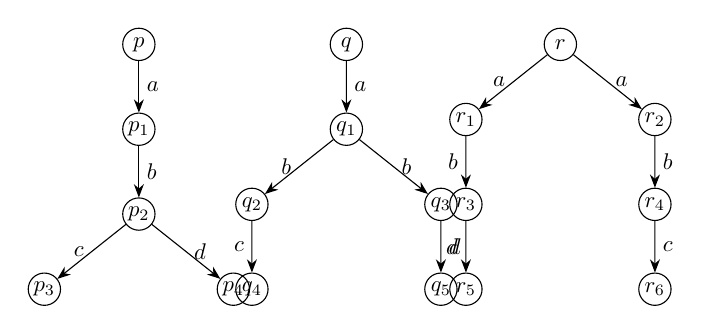
\begin{tikzpicture}[>=Stealth, node distance=8mm and 11mm, every state/.style={minimum size=5mm, inner sep=1pt}, scale=0.82, transform shape]
    \node[state] (p0) {$p$};
    \node[state, below=of p0] (p1) {$p_1$};
    \node[state, below=of p1] (p2) {$p_2$};
    \node[state, below left=of p2] (p3) {$p_3$};
    \node[state, below right=of p2] (p4) {$p_4$};
    \path[->]
        (p0) edge node[right] {$a$} (p1)
        (p1) edge node[right] {$b$} (p2)
        (p2) edge node[left] {$c$} (p3)
        (p2) edge node[right] {$d$} (p4);

    \node[state, right=27mm of p0] (q0) {$q$};
    \node[state, below=of q0] (q1) {$q_1$};
    \node[state, below left=of q1] (q2) {$q_2$};
    \node[state, below right=of q1] (q3) {$q_3$};
    \node[state, below=of q2] (q4) {$q_4$};
    \node[state, below=of q3] (q5) {$q_5$};
    \path[->]
        (q0) edge node[right] {$a$} (q1)
        (q1) edge node[left] {$b$} (q2)
        (q1) edge node[right] {$b$} (q3)
        (q2) edge node[left] {$c$} (q4)
        (q3) edge node[right] {$d$} (q5);

    \node[state, right=28mm of q0] (r0) {$r$};
    \node[state, below left=of r0] (r1) {$r_1$};
    \node[state, below right=of r0] (r2) {$r_2$};
    \node[state, below=of r1] (r3) {$r_3$};
    \node[state, below=of r2] (r4) {$r_4$};
    \node[state, below=of r3] (r5) {$r_5$};
    \node[state, below=of r4] (r6) {$r_6$};
    \path[->]
        (r0) edge node[left] {$a$} (r1)
        (r0) edge node[right] {$a$} (r2)
        (r1) edge node[left] {$b$} (r3)
        (r2) edge node[right] {$b$} (r4)
        (r3) edge node[left] {$d$} (r5)
        (r4) edge node[right] {$c$} (r6);
\end{tikzpicture}
\end{center}

\section{Trace equivalence}

\begin{snippetdefinition}{Traces of a process}
    The set of traces of a process \(q\) is
    \[
        T(q)
        =
        \{a_1\cdots a_n\suchthat
        \exists q_1,\ldots,q_n,
        q\trans{a_1}q_1\trans{a_2}\cdots\trans{a_n}q_n\}.
    \]
    The empty trace is included.
\end{snippetdefinition}

\begin{snippetdefinition}{Trace equivalence}
    Two processes are trace equivalent if
    \[
        p\simeq_T q
        \iff
        T(p)=T(q).
    \]
\end{snippetdefinition}

Two vending machines may have exactly the same observable action sequences while making internal decisions at different points.
For properties depending on what remains possible after an action, trace equivalence is therefore too coarse.

\section{Strong bisimulation}

\begin{snippetdefinition}{Strong bisimulation}
    A relation \(R\subseteq\Proc\cartesianprod\Proc\) is a \emph{strong bisimulation} if, for every \((p,q)\in R\) and every action \(a\):
    \begin{enumerate}
        \item if \(p\trans{a}p'\), then there exists \(q'\) such that
        \[
            q\trans{a}q'
            \qquad\text{and}\qquad
            (p',q')\in R;
        \]
        \item if \(q\trans{a}q'\), then there exists \(p'\) such that
        \[
            p\trans{a}p'
            \qquad\text{and}\qquad
            (p',q')\in R.
        \]
    \end{enumerate}
\end{snippetdefinition}

\begin{snippetdefinition}{Strong bisimilarity}
    Two processes are strongly bisimilar, written
    \[
        p\sim q,
    \]
    if there exists a strong bisimulation \(R\) containing \((p,q)\).
    Equivalently, \(\sim\) is the union of all strong bisimulations.
\end{snippetdefinition}

\begin{snippetexample}{Why the three trace-equivalent processes are not all bisimilar}
    In
    \[
        a.b.(c.0+d.0)
    \]
    after \(a\) and \(b\) the residual state offers both \(c\) and \(d\).
    In a process where the choice between the two branches has already been resolved, the corresponding derivative offers only one of the two actions.
    A bisimulation relation cannot preserve the matching against all choices of an attacker.
\end{snippetexample}

\begin{snippetexample}{A non-functional bisimulation relation}
    A bisimulation between two LTSs can contain, for example,
    \[
        R=\{(p_0,q_0),(p_0,q_2),(p_1,q_1),(p_2,q_1)\}.
    \]
    A single state can therefore be related to several states of the other system: a bisimulation is not a function, but a relation grouping states with the same behaviour.
\end{snippetexample}

\begin{snippettheorem}{Properties of bisimilarity}
    Strong bisimilarity
    \begin{enumerate}
        \item is an equivalence relation;
        \item is the greatest strong bisimulation;
        \item satisfies the local characterization
        \[
            p\sim q
        \]
        if and only if every transition of either process can be matched by the other with bisimilar derivatives.
    \end{enumerate}
\end{snippettheorem}

\begin{snippetexample}{Proving non-bisimilarity}
    Suppose \(p_0\) can perform an action to a state \(p_1\) offering a \(c\)-transition, while every possible matching move of \(q_0\) leads to a state \(q_1\) that cannot perform \(c\).
    Then no bisimulation can contain \((p_0,q_0)\).
\end{snippetexample}

\subsection{Operations on bisimulations}

Consider the relations
\[
    \emptyset,
    \qquad
    \Id,
    \qquad
    \Proc\cartesianprod\Proc,
    \qquad
    R^{-1},
    \qquad
    R\circ S,
    \qquad
    R\union S,
    \qquad
    R\intersection S.
\]
An arbitrary union of bisimulations is again a bisimulation, which justifies defining \(\sim\) as their union.
Intersections do not enjoy the same property in general.

\begin{snippetexercise}{Bisimilarity from a diagram}
    Given an LTS with two initial states \(P,Q\) and several action branches, determine whether they are bisimilar.
    Either construct a relation containing \((P,Q)\), or find a transition forcing a mismatch and use it as a counterexample.
\end{snippetexercise}

\section{Bisimulation game}

The bisimulation game gives a conceptual procedure for proving both bisimilarity and non-bisimilarity.
There are two players:
\begin{itemize}
    \item the attacker chooses one of the two processes and one of its transitions;
    \item the defender must reply with a transition carrying the same label from the other process.
\end{itemize}
The game continues from the pair of derivatives.
If the defender cannot reply, the defender loses; if the defender can reply forever, or the attacker has no move, the defender wins.

\begin{snippettheorem}{}
    \[
        p\sim q
        \iff
        \text{the defender has a winning strategy in the bisimulation game from \((p,q)\)}.
    \]
\end{snippettheorem}

To prove non-bisimilarity it is often easier to describe a winning strategy for the attacker than to enumerate all possible relations, of which there are
\[
    2^{|\Proc|^2}
\]
in the finite case.

\section{Simulation and similarity}

\begin{snippetdefinition}{Simulation}
    A relation \(R\) is a simulation if
    \[
        pRq
        \land
        p\trans{a}p'
        \implies
        \exists q',\ q\trans{a}q'\land p'Rq'.
    \]
    No symmetric condition is required.
\end{snippetdefinition}

Write
\[
    p\sqsubseteq q
\]
if there exists a simulation containing \((p,q)\).
This relation is a preorder and is called \emph{similarity}.

\emph{Double similarity} is defined by
\[
    p\simeq q
    \iff
    p\sqsubseteq q
    \land
    q\sqsubseteq p.
\]
It is coarser than bisimilarity: if \(p\sim q\), then the two processes simulate one another, but the converse can fail because the two simulations may use different relations.

\begin{snippetexample}{Double similarity without bisimilarity}
    Consider processes of the form
    \[
        a.b.0+a.(b.0+c.0)
        \qquad\text{and}\qquad
        a.(b.0+c.0).
    \]
    Each process can simulate the other by choosing a suitable branch, but there is no single symmetric relation satisfying all the matching obligations required by bisimulation.
\end{snippetexample}

\begin{snippetexample}{Simulation and double similarity}
    Similarity \(\sqsubseteq\) is in general a preorder and need not be symmetric.
    Double similarity can equivalently be written as
    \[
        \simeq\;\triangleq\;\sqsubseteq\intersection\sqsubseteq^{-1}.
    \]
    It is symmetric by construction and should not be confused with simulation itself.
\end{snippetexample}

\section{Testing equivalences}

An alternative approach describes behaviour through \emph{observers} or tests.
An observer is a process that interacts with the process under test and has a distinguished success action \(\omega\).
Its action set is therefore
\[
    A_\omega=A\union\{\omega\}.
\]

\subsection{Observations and success}

An observation of \(q\) by \(o\) is a maximal computation of the synchronized system \((q,o)\).
Denote the set of observations by
\[
    \OBS(q,o).
\]
An observation is \emph{successful} if, in one of the reached configurations, the observer can perform \(\omega\).

\begin{snippetdefinition}{May and must testing}
    We say that
    \begin{enumerate}
        \item \(q\) \emph{may pass} \(o\) if at least one observation is successful;
        \item \(q\) \emph{must pass} \(o\) if every maximal observation is successful.
    \end{enumerate}
\end{snippetdefinition}

Two processes are \emph{may equivalent} if they pass exactly the same tests in the may sense, and \emph{must equivalent} if they pass exactly the same tests in the must sense.
Testing equivalence combines the two components.

\begin{snippetexample}{Difference between may and must}
    Processes offering the same traces may be may equivalent because there is always some branch allowing the observer to succeed, but fail to be must equivalent if one process can internally choose a branch from which success becomes impossible.
    In a representative example, \(p\) is may equivalent to \(q\) but not must equivalent, while \(q\) and \(r\) agree with respect to must and hence with respect to the testing equivalence under consideration.
\end{snippetexample}

In that example,
\[
    p\simeq_m q,
    \qquad
    p\not\simeq_M q,
    \qquad
    q\simeq_M r,
    \qquad
    q\simeq_{test}r.
\]

\section{Failures, futures and acceptance sets}

\begin{snippetdefinition}{Refusal and failure}
    A set of actions \(L\) is a \emph{refusal} of a state if the state can refuse every action in \(L\), namely none of them is initially available.
    A \emph{failure} is a pair
    \[
        (s,L)
    \]
    such that after trace \(s\) the process can reach a state refusing \(L\).
\end{snippetdefinition}

Failure equivalence compares sets of failures.
In the setting considered here,
\[
    \text{must equivalence}
    \equiv
    \text{failure equivalence},
\]
whereas
\[
    \text{may equivalence}
    \equiv
    \text{trace equivalence}.
\]

Another description uses \emph{futures}, namely what remains possible after a trace, and acceptance sets.
For a process \(p\),
\[
    \Init(p)=\{a\suchthat\exists p',\ p\trans{a}p'\}
\]
is the set of initially available actions.
Must behaviour can be characterized by comparing, after every trace, the families of action sets that must remain acceptable.

\section{Internal actions and weak equivalences}

Strong bisimulation treats \(\tau\) as an ordinary label and therefore distinguishes internal details that are often intended to be unobservable.
We want to abstract from sequences of internal steps, including internal grinding.

\subsection{Weak transitions}

For a visible action \(a\), define
\[
    \wtrans{a}
    \triangleq
    (\trans{\tau})^*
    \circ
    \trans{a}
    \circ
    (\trans{\tau})^*.
\]
For the empty trace,
\[
    \wtrans{\eps}
    \triangleq
    (\trans{\tau})^*.
\]
More generally, a weak trace allows any number of \(\tau\)-steps before, after, and between visible actions.

\begin{snippetdefinition}{Weak trace equivalence}
    Two processes are weak trace equivalent if they have the same sets of visible traces when \(\tau\)-steps are ignored.
\end{snippetdefinition}

Testing can similarly be weakened by allowing the process and observer to perform independent internal steps between visible synchronizations.

\subsection{Weak bisimulation}

A general formulation matches weak transitions for arbitrary traces.
The following local characterization is sufficient.
Define
\[
    \widehat\mu
    =
    \begin{cases}
        \eps & \mu=\tau,\\
        \mu & \mu\neq\tau.
    \end{cases}
\]

\begin{snippetdefinition}{Weak bisimulation}
    A symmetric relation \(R\) is a weak bisimulation if
    \[
        pRq
        \land
        p\trans{\mu}p'
    \]
    implies the existence of \(q'\) such that
    \[
        q\wtrans{\widehat\mu}q'
        \qquad\text{and}\qquad
        p'Rq'.
    \]
    Weak bisimilarity is written
    \[
        p\approx q.
    \]
\end{snippetdefinition}

Processes differing only by redundant internal steps can therefore be weakly bisimilar.
Weak bisimulation nevertheless preserves visible branching structure and does not collapse all distinctions in the way trace equivalence does.

\subsection{Branching bisimulation}

Branching bisimulation preserves more precisely the point at which an observable choice is resolved.

\begin{snippetdefinition}{Branching bisimulation}
    A symmetric relation \(R\) is a branching bisimulation if, whenever
    \[
        pRq
        \qquad\text{and}\qquad
        p\trans{\mu}p',
    \]
    one of the following holds:
    \begin{enumerate}
        \item \(\mu=\tau\) and \(p'Rq\);
        \item there exist \(q'',q'\) such that
        \[
            q\wtrans{\eps}q''\trans{\mu}q',
        \]
        with
        \[
            pRq'',
            \qquad
            p'Rq'.
        \]
    \end{enumerate}
\end{snippetdefinition}

Intermediate states traversed through \(\tau\)-steps before the matching action must therefore remain related to the source state, preserving the branching structure.

\begin{snippetexample}{Testing and bisimulation do not coincide}
    There are complementary counterexamples.
    In one, two systems are weakly testing equivalent but are neither weakly bisimilar nor branching bisimilar.
    In another, two systems containing a \(\tau\)-loop are weakly and branching bisimilar but not testing equivalent.
    Thus testing-based observational notions and branching-matching notions are incomparable in general.
\end{snippetexample}

\subsection{The spectrum of equivalences}

The equivalences form a spectrum.
Strong bisimilarity is among the finest notions; branching and weak bisimilarity progressively abstract from internal steps; failure/must, trace/may, and other linear-time equivalences are coarser.
For strongly convergent systems, the corresponding strong and weak notions collapse in the expected way, in particular must with failures and may with traces.
The appropriate equivalence therefore depends on which aspects of behaviour are intended to remain observable.

\pagebreak
\part{CCS}

\section{A Calculus for Communicating Systems}

CCS collects in a single language the main ingredients introduced so far: LTSs as behavioural models, process-composition operators, SOS rules, and behavioural equivalences.
Its sequential fragment contains the nil process, action prefixing, process names with recursive definitions, and nondeterministic choice.
Using these operators, every finite LTS can be described up to isomorphism.
Adding parallel composition, restriction, and relabelling yields a language for communicating systems.

\subsection{Names, co-names and actions}

Let \(\mathcal A\) be a set of channel names.
For every \(a\in\mathcal A\), there is a co-name \(\overline a\).
Put
\[
    \mathcal L
    =
    \mathcal A\union\overline{\mathcal A},
    \qquad
    \Act
    =
    \mathcal L\union\{\tau\}.
\]
Complementation satisfies
\[
    \overline{\overline a}=a,
    \qquad
    \overline\tau=\tau.
\]
Let \(\mathcal K\) be a set of process constants.

\subsection{Syntax}

The syntax of CCS is
\[
    P
    ::=K
    \mid \alpha.P
    \mid \sum_{i\in I}P_i
    \mid P_1\mid P_2
    \mid P\setminus L
    \mid P[f],
\]
where
\[
    K\in\mathcal K,
    \qquad
    \alpha\in\Act,
    \qquad
    L\subseteq\mathcal A,
\]
and \(f\) is a relabelling function preserving \(\tau\) and complementation:
\[
    f(\tau)=\tau,
    \qquad
    f(\overline a)=\overline{f(a)}.
\]

Binary choice is
\[
    P+Q
    \triangleq
    \sum_{i\in\{1,2\}}P_i,
\]
while
\[
    \nil
    \triangleq
    \sum_{i\in\emptyset}P_i.
\]
The usual precedence conventions bind restriction and relabelling most tightly, then prefixing, then parallel composition, and finally summation.

A process constant is equipped with a defining equation
\[
    K\triangleq P.
\]
Definitions may be recursive, for example
\[
    A\triangleq a.A\mid A.
\]

\section{SOS of CCS}

The states of the CCS LTS are process terms and its labels are the actions in \(\Act\).
The main SOS rules are the following.

\subsection{Prefix and summation}

\[
    \frac{}{\alpha.P\trans{\alpha}P}
    \tag{ACT}
\]

For summation,
\[
    \frac{P_j\trans{\alpha}P'}
    {\sum_{i\in I}P_i\trans{\alpha}P'}
    \qquad j\in I.
    \tag{SUM}
\]

\subsection{Parallel composition}

Independent moves are described by
\[
    \frac{P\trans{\alpha}P'}
    {P\mid Q\trans{\alpha}P'\mid Q},
    \tag{COM1}
\]
\[
    \frac{Q\trans{\alpha}Q'}
    {P\mid Q\trans{\alpha}P\mid Q'}.
    \tag{COM2}
\]
Synchronization is
\[
    \frac{P\trans{a}P'\qquad Q\trans{\overline a}Q'}
    {P\mid Q\trans{\tau}P'\mid Q'}.
    \tag{COM3}
\]

\begin{snippetexample}{Parallel composition of complementary prefixes}
    The process
    \[
        a.\nil\mid\overline a.\nil
    \]
    can
    \begin{enumerate}
        \item perform \(a\) independently;
        \item perform \(\overline a\) independently;
        \item synchronize the two actions and perform
        \[
            a.\nil\mid\overline a.\nil
            \trans{\tau}
            \nil\mid\nil.
        \]
    \end{enumerate}
\end{snippetexample}

\subsection{Restriction}

\[
    \frac{P\trans{\alpha}P'\qquad
    \alpha,\overline\alpha\notin L}
    {P\setminus L\trans{\alpha}P'\setminus L}.
    \tag{RES}
\]
A restricted name and its co-name cannot be exposed independently to the environment.
Internal \(\tau\)-actions are not blocked.

\subsection{Relabelling}

\[
    \frac{P\trans{\alpha}P'}
    {P[f]\trans{f(\alpha)}P'[f]}.
    \tag{REL}
\]

\subsection{Constants}

If
\[
    K\triangleq P
\]
and \(P\trans{\alpha}P'\), then
\[
    \frac{P\trans{\alpha}P'}{K\trans{\alpha}P'}.
    \tag{CON}
\]

\begin{snippetexample}{An SOS derivation}
    Let
    \[
        A\triangleq a.A.
    \]
    A transition of a compound term such as
    \[
        ((A\mid a.\nil)\mid b.\nil)[c/a]
    \]
    is derived by first obtaining an \(a\)-transition from the selected component, lifting it through the parallel compositions, and finally applying the relabelling, which changes the label into \(c\).
\end{snippetexample}

\section{The 50 prisoners problem}

CCS can be used to model the well-known 50 prisoners problem.
There are fifty prisoners. One at a time, according to a fair schedule, they are taken to a room containing a light bulb whose initial state is unknown.
At some point a prisoner may declare that every prisoner has already visited the room; an incorrect declaration makes all prisoners lose.

\subsection{A first model}

Assume first that the light is initially on.
One possible light process is
\[
    \mathsf{Light}
    \triangleq
    \mathsf{turnOff}.\mathsf{turnOn}.\mathsf{Light}.
\]
A counter can initially be represented by
\[
    C_{i+1}
    \triangleq
    \mathsf{turnOff}.C_i
    +
    \tau.C_{i+1},
    \qquad
    C_0\triangleq\mathsf{freeAll}.
\]
A generic prisoner may have a phase in which the light is turned on once, followed by a phase in which the prisoner no longer contributes:
\[
    P\triangleq\mathsf{turnOn}.IP+\tau.P,
    \qquad
    IP\triangleq\tau.IP.
\]
This model has a problem: prisoners may always select \(\tau\) and never interact with the light.
Replace the inactive branches by actions that respect the light state:
\[
    C_{i+1}
    \triangleq
    \mathsf{turnOff}.C_i
    +
    \mathsf{turnOn}.\mathsf{turnOff}.C_{i+1},
\]
\[
    P
    \triangleq
    \mathsf{turnOn}.IP
    +
    \mathsf{turnOff}.\mathsf{turnOn}.P,
    \qquad
    IP\triangleq\tau.IP.
\]
The complete system is obtained by putting the light, the counter, and the prisoners in parallel and restricting the channels \(\mathsf{turnOn}\) and \(\mathsf{turnOff}\).

The model still exposes two issues.
A prisoner may perform internal behaviour indefinitely, so fairness must be represented correctly.
Moreover, the fact that only one prisoner at a time can be in the room must be modelled explicitly.

\subsection{Mutual exclusion}

Introduce a room process
\[
    \mathsf{Room}
    \triangleq
    \mathsf{roomIn}.\mathsf{roomOut}.\mathsf{Room}.
\]
Expand the prisoners with synchronization actions for entering and leaving the room.
Mutual exclusion is then enforced by handshake communication rather than assumed implicitly.

In particular,
\[
    C_{i+1}
    \triangleq
    \mathsf{roomIn}.(
      \mathsf{turnOff}.\mathsf{roomOut}.C_i
      +
      \mathsf{turnOn}.\mathsf{turnOff}.\mathsf{roomOut}.C_{i+1}),
\]
\[
    P\triangleq
    \mathsf{roomIn}.(
      \mathsf{turnOn}.\mathsf{roomOut}.IP
      +
      \mathsf{turnOff}.\mathsf{turnOn}.\mathsf{roomOut}.P),
\]
\[
    IP\triangleq\mathsf{roomIn}.\tau.\mathsf{roomOut}.IP.
\]
The complete system restricts
\[
    \{\mathsf{turnOn},\mathsf{turnOff},\mathsf{roomIn},\mathsf{roomOut}\}.
\]

\subsection{Unknown initial state}

If the initial state of the bulb is unknown, model the light by
\[
    \mathsf{Light}
    \triangleq
    \tau.\mathsf{LightOn}+\tau.\mathsf{LightOff},
\]
\[
    \mathsf{LightOn}\triangleq\mathsf{turnOff}.\mathsf{LightOff},
    \qquad
    \mathsf{LightOff}\triangleq\mathsf{turnOn}.\mathsf{LightOn}.
\]
The counter cannot know whether the first switch-off corresponds to an actual contribution from another prisoner.
The ambiguity can be removed by making every non-counter prisoner contribute twice and having the counter count \(98\) switch-offs.
Indeed,
\[
    50+49=99,
    \qquad
    49+49=98,
\]
whereas if at least one prisoner had never entered, the maximum would be
\[
    49+48=97
\]
with the light initially on, or \(48+48=96\) at the other extreme.
Thus define
\[
    P\triangleq
    \mathsf{roomIn}.(
      \mathsf{turnOn}.\mathsf{roomOut}.RP
      +
      \mathsf{turnOff}.\mathsf{turnOn}.\mathsf{roomOut}.P),
\]
\[
    RP\triangleq
    \mathsf{roomIn}.(
      \mathsf{turnOn}.\mathsf{roomOut}.IP
      +
      \mathsf{turnOff}.\mathsf{turnOn}.\mathsf{roomOut}.RP),
\]
\[
    IP\triangleq\mathsf{roomIn}.\tau.\mathsf{roomOut}.IP,
\]
and use \(C_{98}\) in the full system.

\section{Value-passing CCS}

In value-passing CCS, a handshake transfers data as well as control.
For instance, a bank process may receive a request carrying an identifier or an amount, process the value, and reply on the complementary channel.

Value-passing CCS can be encoded in standard CCS by replacing a parameterized input with a sum, possibly infinite, over all values:
\[
    a(x).P
    \quad\leadsto\quad
    \sum_{v\in V}a(v).P\{v/x\}.
\]
This translation may produce an infinite LTS from a compact syntactic description.
CCS is expressive enough to be Turing complete.

\begin{snippetexample}{Bank}
    Consider
    \[
        \overline{\mathsf{pay}}(6).0
        \mid
        \mathsf{pay}(x).\overline{\mathsf{save}}(x/2).0
        \mid
        \mathsf{Bank}(100).
    \]
    After synchronization on \(\mathsf{pay}\), the second process becomes \(\overline{\mathsf{save}}(3).0\); a second synchronization leads to \(\mathsf{Bank}(103)\), where
    \[
        \mathsf{Bank}(total)
        \triangleq
        \mathsf{save}(x).\mathsf{Bank}(total+x).
    \]
\end{snippetexample}

\section{Buffers and bisimilarity}

\subsection{Finite-capacity buffers}

A buffer of capacity \(1\) can be defined by
\[
    B_0^1\triangleq\mathsf{in}.B_1^1,
    \qquad
    B_1^1\triangleq\mathsf{out}.B_0^1.
\]
For capacity \(n\):
\begin{align*}
    B_0^n&\triangleq\mathsf{in}.B_1^n,\\
    B_n^n&\triangleq\mathsf{out}.B_{n-1}^n,\\
    B_i^n&\triangleq
    \mathsf{in}.B_{i+1}^n
    +
    \mathsf{out}.B_{i-1}^n,
    \qquad 0<i<n.
\end{align*}

\begin{snippettheorem}{}
    A buffer of capacity \(n\) is strongly bisimilar to \(n\) one-place buffers in parallel:
    \[
        B_0^n
        \sim
        \underbrace{B_0^1\mid\cdots\mid B_0^1}_{n\text{ copies}}.
    \]
\end{snippettheorem}

\begin{snippetproof}{Relation based on total occupancy}
    In the parallel composition of \(n\) cells, every component is either empty or full.
    Relate \(B_i^n\) with all parallel configurations containing exactly \(i\) full cells.
    An \(\mathsf{in}\)-action increases occupancy by one in both systems, and an \(\mathsf{out}\)-action decreases it by one.
    The resulting relation is a bisimulation.
\end{snippetproof}

\begin{snippetexercise}{}
    Prove the usual equivalence properties of bisimilarity and show
    \[
        B_0^{n+k}
        \sim
        B_0^n\mid B_0^k.
    \]
\end{snippetexercise}

\subsection{A digression on ``advanced proof methods''}

The following humorous list illustrates methods that are not substitutes for a proof:
\begin{enumerate}
    \item proof by obviousness: ``so evident it needs not to be mentioned'';
    \item proof by general agreement: ``all in favor?'';
    \item proof by majority, when general agreement is unavailable;
    \item proof by plausibility: ``it sounds good'';
    \item proof by intuition: ``I have this feeling...'';
    \item proof by lost reference: ``I saw it somewhere'';
    \item proof by obscure reference: an untraceable citation in old proceedings;
    \item proof by logic: ``it is in the textbook, hence it must be true'';
    \item proof by intimidation: ``who is saying that it is false!?'';
    \item proof by authority: ``Don Knuth said it was true'';
    \item proof by deception: ``everybody please turn their backs...'';
    \item proof by divine word: ``Lord said let it be true''.
\end{enumerate}
For bisimulation, the actual relation must be exhibited and its matching conditions checked; intuition from a picture does not replace the proof.

\section{Congruence of strong bisimilarity}

\begin{snippettheorem}{Congruence theorem}
    Strong bisimilarity is preserved by CCS operators.
    If \(P\sim Q\), then for every appropriate context,
    \begin{align*}
        \alpha.P&\sim\alpha.Q,\\
        P+R&\sim Q+R,\\
        P\mid R&\sim Q\mid R,\\
        P\setminus L&\sim Q\setminus L,\\
        P[f]&\sim Q[f].
    \end{align*}
\end{snippettheorem}

The standard proof technique extends the original bisimulation with pairs obtained by placing related processes in the same context, and then checks the SOS rules.

For choice, this yields algebraic laws such as
\[
    P+Q\sim Q+P,
\]
\[
    (P+Q)+R\sim P+(Q+R),
\]
\[
    P+\nil\sim P,
\]
\[
    P+P\sim P.
\]
For parallel composition,
\[
    P\mid0\sim P,
    \qquad
    P\mid Q\sim Q\mid P,
    \qquad
    (P\mid Q)\mid R\sim P\mid(Q\mid R).
\]

\begin{snippetproof}{Commutativity of choice}
    Consider
    \[
        R=\Id\union\{(P+Q,Q+P)\suchthat P,Q\in\Proc\}.
    \]
    Every transition of \(P+Q\) originates from either \(P\) or \(Q\); the same transition is available in \(Q+P\) through the symmetric summation rule and has the same derivative.
    The converse direction is identical, so \(R\) is a bisimulation.
\end{snippetproof}

\section{Cells and FIFO buffers}

We compare different ways of building memory and buffers.

\subsection{Cells}

A one-place cell has two conceptual states, empty and full:
\[
    \mathsf{Empty}\trans{\mathsf{in}}\mathsf{Full},
    \qquad
    \mathsf{Full}\trans{\mathsf{out}}\mathsf{Empty}.
\]
A capacity-two cell has three occupancy levels.
Compare:
\begin{enumerate}
    \item a directly defined cell of capacity two;
    \item \(\mathsf{ParCell}=\mathsf{Cell}_1\mid\mathsf{Cell}_1\);
    \item \(\mathsf{SeqCell}\), obtained by linking two cells in series through a private channel \(p\).
\end{enumerate}
Determine which constructions are equivalent under the behavioural equivalences introduced earlier.

\subsection{FIFO with binary data}

For values \(0,1\), a capacity-one FIFO distinguishes the states \([]\), \([0]\), and \([1]\).
A capacity-two FIFO has states
\[
    [],[0],[1],[00],[10],[01],[11]
\]
with actions \(\mathsf{in0}\), \(\mathsf{in1}\), \(\mathsf{out0}\), and \(\mathsf{out1}\) respecting FIFO order.
Compare the direct FIFO with
\[
    \mathsf{ParFIFO}=\mathsf{FIFO}_1\mid\mathsf{FIFO}_1
\]
and with a serial composition using private channels \(p_0,p_1\).
Two independent cells in parallel do not automatically preserve data order, whereas a serial connection can.

\section{Weak bisimilarity in CCS}

Recall
\[
    \wtrans{a}
    =
    (\trans{\tau})^*\circ\trans{a}\circ(\trans{\tau})^*,
    \qquad a\neq\tau,
\]
and
\[
    \wtrans{\eps}
    =
    (\trans{\tau})^*.
\]
Moreover, put
\[
    \widehat a=a,
    \qquad
    \widehat\tau=\eps.
\]

Weak bisimulation uses \(\wtrans{\widehat\mu}\) to match a transition labelled \(\mu\).
Typical equivalences include
\[
    a.\tau.P\approx a.P,
\]
as well as other laws eliminating redundant internal steps or unobservable internal loops.

Weak bisimilarity is an equivalence relation, but it is not a congruence for choice \(+\).
It is preserved by the other CCS operators under the usual conditions.
This failure for choice motivates the introduction of observational congruence in the axiomatization of weak equivalences.

\section{A communication protocol}

Consider the abstract specification
\[
    \mathsf{Spec}
    \triangleq
    \mathsf{acc}.\mathsf{del}.\mathsf{Spec}.
\]
The implementation is
\[
    \mathsf{Impl}
    =
    (\mathsf{Send}\mid\mathsf{Med}\mid\mathsf{Rec})
    \setminus
    \{\mathsf{send},\mathsf{trans},\mathsf{ack},\mathsf{error}\}.
\]
The components are
\begin{align*}
    \mathsf{Send}&\triangleq\mathsf{acc}.\mathsf{Sending},\\
    \mathsf{Sending}&\triangleq\mathsf{send}.\mathsf{Wait},\\
    \mathsf{Wait}&\triangleq
        \mathsf{ack}.\mathsf{Send}
        +
        \mathsf{error}.\mathsf{Sending},\\
    \mathsf{Rec}&\triangleq\mathsf{trans}.\mathsf{Del},\\
    \mathsf{Del}&\triangleq\mathsf{del}.\mathsf{Ack},\\
    \mathsf{Ack}&\triangleq\mathsf{ack}.\mathsf{Rec},\\
    \mathsf{Med}&\triangleq\mathsf{send}.\mathsf{Med}_0,\\
    \mathsf{Med}_0&\triangleq
        \tau.\mathsf{Err}
        +
        \mathsf{trans}.\mathsf{Med},\\
    \mathsf{Err}&\triangleq\mathsf{error}.\mathsf{Med}.
\end{align*}
The medium can either deliver the message correctly or report an error, in which case the sender retries.

\begin{snippetexercise}{Correctness of the protocol}
    Draw the LTSs of \(\mathsf{Spec}\) and \(\mathsf{Impl}\), and prove
    \[
        \mathsf{Impl}\approx\mathsf{Spec}.
    \]
    The proof must abstract from the internal send, transmission, acknowledgement, and error steps, leaving externally only the cycle \(\mathsf{acc}.\mathsf{del}\).
\end{snippetexercise}

\pagebreak
\part{Equational axiomatizations}

\section{Why axiomatize an equivalence}

Checking directly whether two process terms are equivalent can be expensive: their LTSs must be constructed and then an appropriate behavioural-equivalence relation must be established.
An equational axiomatization allows us instead to reason syntactically on terms, often avoiding the explicit computation of LTSs and bisimulation relations.
This is useful for automated reasoning and also gives a deeper understanding of the semantic effect of an equivalence.

We seek an equational theory \(E_{CCS}\) such that
\[
    E_{CCS}\vdash P=Q
\]
is sound and complete for strong bisimilarity.

\begin{snippetdefinition}{Soundness and completeness}
    An axiomatization \(E\) is
    \begin{enumerate}
        \item \emph{sound} for \(\sim\) if
        \[
            E\vdash P=Q
            \implies
            P\sim Q;
        \]
        \item \emph{complete} for \(\sim\) if
        \[
            P\sim Q
            \implies
            E\vdash P=Q.
        \]
    \end{enumerate}
\end{snippetdefinition}

Soundness ensures that the axioms never identify terms belonging to different bisimulation classes.
Completeness ensures that every pair of bisimilar terms can be equated by equational reasoning.
We will seek analogous results for weak equivalences.

\section{Equational logic}

\subsection{Signatures and terms}

A signature \(\Sigma\) contains function symbols with fixed arities; symbols of arity zero are constants.
Write
\[
    T(\Sigma)
\]
for the set of terms, possibly containing variables, and
\[
    CT(\Sigma)
\]
for the set of closed terms.

A substitution maps variables to terms and extends homomorphically to all terms.
A \emph{closed substitution} maps every variable to a closed term.
We write
\[
    t\{u/x\}
\]
for substituting \(u\) for \(x\), and similarly for simultaneous substitutions.

\begin{snippetdefinition}{Axiom system}
    An equational axiomatization \(E\) is a set of equations
    \[
        s=t
    \]
    between terms over the signature.
    It is finite if it contains finitely many axioms.
\end{snippetdefinition}

The derivable equality \(=_E\) is the least relation containing every substitution instance of the axioms and closed under:
\begin{enumerate}
    \item reflexivity;
    \item symmetry;
    \item transitivity;
    \item substitution;
    \item contexts, namely replacing equals by equals inside the same operator.
\end{enumerate}

Equational logic can therefore be presented by the usual inference rules
\[
    \frac{}{t=t},
    \qquad
    \frac{t=u}{u=t},
    \qquad
    \frac{t=u\qquad u=v}{t=v},
\]
together with congruence rules for the function symbols and substitution instances of the axioms.

\section{Axioms for Basic CCS}

For the fragment with \(\nil\), prefixing, and summation, the basic axioms are
\begin{align*}
    A1\qquad& P+Q = Q+P,\\
    A2\qquad& (P+Q)+R = P+(Q+R),\\
    A3\qquad& P+\nil = P,\\
    A4\qquad& P+P = P.
\end{align*}
Thus \(+\) behaves like idempotent union of initial alternatives.

\begin{snippetexample}{Equational calculation}
    Consider
    \begin{align*}
        a.(b.\nil+\nil)+(a.\nil+a.b.\nil)
        &=a.b.\nil+(a.\nil+a.b.\nil) && (A3)\\
        &=a.b.\nil+(a.b.\nil+a.\nil) && (A1)\\
        &=(a.b.\nil+a.b.\nil)+a.\nil && (A2)\\
        &=a.b.\nil+a.\nil && (A4).
    \end{align*}
    Hence
    \[
        \mathsf{BaseAX}\vdash
        a.(b.\nil+\nil)+(a.\nil+a.b.\nil)
        =a.b.\nil+a.\nil.
    \]
\end{snippetexample}

\section{Restriction and relabelling}

Restriction and relabelling can be pushed through summation and underneath prefixes by equational laws.
For restriction:
\begin{align*}
    \nil\setminus L &= \nil,\\
    (P+Q)\setminus L &= P\setminus L+Q\setminus L,\\
    (\alpha.P)\setminus L
    &=
    \begin{cases}
        \alpha.(P\setminus L) & \alpha,\overline\alpha\notin L,\\
        \nil & \text{if the action is blocked by \(L\)}.
    \end{cases}
\end{align*}
For relabelling:
\begin{align*}
    \nil[f]&=\nil,\\
    (P+Q)[f]&=P[f]+Q[f],\\
    (\alpha.P)[f]&=f(\alpha).P[f].
\end{align*}
These laws eliminate structural operators by pushing them towards the inside of a term.

\section{Expansion theorem}

Parallel composition can be eliminated equationally by expanding its possible initial moves.
Suppose
\[
    P=\sum_{i\in I}\alpha_i.P_i,
    \qquad
    Q=\sum_{j\in J}\beta_j.Q_j.
\]
Then the expansion law has the form
\[
    P\mid Q
    =
    \sum_{i\in I}\alpha_i.(P_i\mid Q)
    +
    \sum_{j\in J}\beta_j.(P\mid Q_j)
    +
    \sum_{\substack{i\in I,j\in J\\\alpha_i=\overline{\beta_j}}}
        \tau.(P_i\mid Q_j).
\]
The first two groups represent independent moves; the last group represents synchronizations.

\begin{snippetexample}{Expansion with synchronization}
    Let
    \[
        p=\alpha.p'+\beta.p'',
        \qquad
        q=\overline\alpha.q'+\gamma.q''.
    \]
    The expansion of \(p\mid q\) contains the independent moves \(\alpha,\beta,\overline\alpha,\gamma\), and the synchronization summand
    \[
        \tau.(p'\mid q').
    \]
    If channel \(\alpha\) is then restricted, the external \(\alpha\)- and \(\overline\alpha\)-moves disappear while the internal \(\tau\)-move remains possible.
\end{snippetexample}

\section{Soundness for strong bisimilarity}

\begin{snippettheorem}{Soundness}
    The axioms for Basic CCS, restriction, relabelling, and expansion are sound for strong bisimilarity.
    Therefore,
    \[
        E_{CCS}\vdash P=Q
        \implies
        P\sim Q.
    \]
\end{snippettheorem}

The proof has two levels.
First, check that both sides of every axiom are strongly bisimilar.
Then use the fact that \(\sim\) is an equivalence relation and a congruence: every rule of equational logic therefore preserves bisimilarity.

\section{Completeness for finite CCS}

\subsection{Standard form}

\begin{snippetdefinition}{Standard form}
    A finite process is in \emph{standard form} if it has the shape
    \[
        \sum_{i=1}^m\mu_i.P_i
    \]
    and every derivative \(P_i\) is itself in standard form, recursively down to \(\nil\).
\end{snippetdefinition}

Using the axioms for restriction, relabelling, and expansion, every recursion-free CCS term can be transformed equationally into standard form.

Define the maximum depth \(d(P)\) as the maximum length of a computation of the finite process \(P\).

\begin{snippettheorem}{Completeness for strong bisimilarity}
    For finite CCS processes,
    \[
        P\sim Q
        \implies
        E_{CCS}\vdash P=Q.
    \]
\end{snippettheorem}

\begin{snippetproof}{Idea}
    Put both processes in standard form:
    \[
        P=\sum_i\mu_i.P_i,
        \qquad
        Q=\sum_j\nu_j.Q_j.
    \]
    Proceed by induction on the maximum depth.
    By bisimilarity, every summand \(\mu_i.P_i\) of \(P\) must be matched by a summand \(\mu_i.Q_j\) of \(Q\) such that
    \[
        P_i\sim Q_j.
    \]
    By the induction hypothesis,
    \[
        E_{CCS}\vdash P_i=Q_j.
    \]
    Thus every summand of \(P\) is equationally represented in \(Q\).
    The symmetric argument covers the summands of \(Q\), and idempotence \(A4\) removes duplicates.
\end{snippetproof}

\section{Weak equivalences and observational congruence}

Weak bisimilarity \(\approx\) is not a congruence for \(+\).
For a compositional equational theory we therefore consider the greatest congruence contained in \(\approx\), called \emph{observational congruence}.

\begin{snippetdefinition}{Observational congruence}
    Two processes \(p,q\) are observationally congruent, written here
    \[
        p\simeq_c q,
    \]
    if every immediate transition
    \[
        p\trans{\mu}p'
    \]
    can be matched by the appropriate weak transition of \(q\), respecting the initial observation, to a derivative \(q'\) satisfying
    \[
        p'\approx q',
    \]
    and symmetrically for transitions of \(q\).
\end{snippetdefinition}

The distinction from weak bisimulation is especially important for an initial \(\tau\)-transition: observational congruence does not allow it to be discarded arbitrarily inside a choice context.
We have
\[
    \sim\ \subseteq\ \simeq_c\ \subseteq\ \approx.
\]

\begin{snippettheorem}{Hennessy's lemma}
    If \(p\approx q\), then at least one of the following holds:
    \[
        p\simeq_c q,
        \qquad
        \tau.p\simeq_c q,
        \qquad
        p\simeq_c\tau.q.
    \]
\end{snippettheorem}

\section{Tau laws}

The weak axiomatization adds the laws
\begin{align*}
    \tau1\qquad&\mu.\tau.P = \mu.P,\\
    \tau2\qquad&P+\tau.P = \tau.P,\\
    \tau3\qquad&\mu.(P+\tau.Q)
        =
        \mu.(P+\tau.Q)+\mu.Q.
\end{align*}
These equations saturate a term with respect to weakly reachable behaviour.

\subsection{Full standard form}

A standard form is \emph{full} if it explicitly contains all summands corresponding to the relevant weak transitions: if
\[
    P\wtrans{\mu}P',
\]
then the form contains, up to the equational theory, the appropriate direct summand \(\mu.P'\).

\begin{snippetproposition}{Saturation lemma}
    If \(P\) is in standard form and
    \[
        P\wtrans{\mu}P',
    \]
    then the axioms \(\tau1,\tau2,\tau3\) allow us to derive
    \[
        P=P+\mu.P'
    \]
    in the form required by the observational semantics.
\end{snippetproposition}

\begin{snippetproof}{}
    Proceed by induction on the depth of \(P\). Since \(P\) is in standard form and \(P\wtrans{\mu}P'\), consider the following cases.
    \begin{enumerate}
        \item If \(\mu.P'\) is already a summand of \(P\), then
        \[
            P=P+\mu.P'
        \]
        follows directly from \(A4\).

        \item Suppose \(\mu.Q\) is a summand of \(P\) and
        \[
            Q\wtrans{\tau}P'.
        \]
        By the induction hypothesis,
        \[
            EQ_\tau\vdash Q=Q+\tau.P'.
        \]
        Hence
        \begin{align*}
            P&=P+\mu.Q &&(A4)\\
             &=P+\mu.(Q+\tau.P') &&(EQ_\tau\vdash Q=Q+\tau.P')\\
             &=P+\mu.(Q+\tau.P')+\mu.P' &&(\tau3)\\
             &=P+\mu.Q+\mu.P' &&(EQ_\tau\vdash Q=Q+\tau.P')\\
             &=P+\mu.P' &&(A4).
        \end{align*}

        \item Suppose \(\tau.Q\) is a summand of \(P\) and
        \[
            Q\wtrans{\mu}P'.
        \]
        By the induction hypothesis \(EQ_\tau\vdash Q=Q+\mu.P'\), and
        \begin{align*}
            P&=P+\tau.Q &&(A4)\\
             &=P+\tau.Q+Q &&(\tau2)\\
             &=P+\tau.Q+Q+\mu.P' &&(EQ_\tau\vdash Q=Q+\mu.P')\\
             &=P+\tau.Q+\mu.P' &&(\tau2)\\
             &=P+\mu.P' &&(A4).
        \end{align*}
    \end{enumerate}
\end{snippetproof}

Every standard form can therefore be transformed into a full standard form without changing the relevant depth.

\begin{snippetproof}{Reduction to full standard form}
    Proceed by induction on the depth of \(P\). At depth zero, \(P\equiv\nil\).
    Otherwise, recursively transform every continuation of the summands of \(P\) into full standard form without increasing its depth.
    Then consider all pairs \((\mu_i,P_i)\) such that
    \[
        P\wtrans{\mu_i}P_i
        \qquad\text{but}\qquad
        P\not\trans{\mu_i}P_i.
    \]
    By the saturation lemma, all missing summands can be added equationally:
    \[
        EQ_\tau\vdash
        P=P+\mu_1.P_1+\cdots+\mu_k.P_k.
    \]
    The right-hand side is in full standard form and has the same depth as \(P\).
\end{snippetproof}

\begin{snippettheorem}{Weak completeness}
    The axiomatization obtained by adding the tau laws is sound and complete for observational congruence on finite processes.
\end{snippettheorem}

\begin{snippetproof}{Idea}
    Put two observationally congruent terms in full standard form and proceed by induction on depth.
    Hennessy's lemma reduces the comparison of weakly bisimilar derivatives to three observational-congruence cases, possibly prefixing one derivative by \(\tau\).
    The tau laws and the induction hypothesis then match all summands of the two forms; associativity, commutativity, and idempotence conclude the equational equality.
\end{snippetproof}

More precisely, if \(\mu.P'\) is a summand of \(P\), observational congruence and the full standard form of \(Q\) yield a summand \(\mu.Q'\) with \(P'\approx Q'\).
By Hennessy's lemma there are three cases:
\begin{enumerate}
    \item \(P'\simeq_c Q'\): the induction hypothesis gives directly \(EQ_\tau\vdash P'=Q'\);
    \item \(P'\simeq_c\tau.Q'\): reduce \(\tau.Q'\) to full standard form, apply induction, and then use \(\tau1\) to derive \(EQ_\tau\vdash\mu.P'=\mu.Q'\);
    \item \(\tau.P'\simeq_c Q'\): symmetric to the previous case.
\end{enumerate}
Repeat the argument for every summand of \(Q\); \(A4\) removes duplicates.

\pagebreak
\part{Modal logics and model checking}

\section{Equivalence checking and model checking}

Let \(\mathit{Impl}\) be an implementation of a reactive system, for example a process written in CCS.
There are two basic approaches to the verification of its correctness.

In \emph{equivalence checking} we compare the implementation with a complete behavioural specification:
\[
    \mathit{Impl} \equiv \mathit{Spec},
\]
where \(\equiv\) is an abstract behavioural equivalence, for example strong or weak bisimilarity.
The specification is usually expressed in the same language as the implementation and describes the whole intended behaviour.

In \emph{model checking} we verify one particular property:
\[
    \mathit{Impl} \models F.
\]
Here \(\models\) is a satisfaction relation and \(F\) is a property, usually expressed by a logic.
Thus a logical formula gives a partial specification of the intended behaviour.

\subsection{Modal and temporal properties}

A modal property describes what a system can or must do from its current state.
A temporal property describes how a property behaves along the possible evolutions of the system.
Typical properties of reactive systems include:
\begin{itemize}
    \item \emph{safety}: something bad never happens;
    \item \emph{liveness}: something good eventually happens;
    \item \emph{possibility}: a state satisfying a property can be reached;
    \item \emph{inevitability}: all reachable states satisfy a property.
\end{itemize}

\section{Hennessy--Milner Logic}

\subsection{Syntax}

\begin{snippetdefinition}{Hennessy--Milner Logic}
    Let \(\Act\) be the set of actions of an LTS.
    The formulae of Hennessy--Milner Logic are generated by
    \[
        F,G ::= \ttt \mid \fff \mid F\land G \mid F\lor G
        \mid \langle a\rangle F \mid [a]F,
        \qquad a\in\Act.
    \]
    The modality \(\langle a\rangle F\) is a \emph{possibility}: the process can perform an \(a\)-action and reach a process satisfying \(F\).
    The modality \([a]F\) is a \emph{necessity}: every \(a\)-derivative, if any, satisfies \(F\).
\end{snippetdefinition}

In particular,
\[
    \langle a\rangle\ttt
\]
expresses the capability of performing an \(a\)-action, whereas
\[
    [a]\fff
\]
expresses the inability to perform an \(a\)-action.
For example,
\[
    \langle\mathsf{coin}\rangle
    \bigl(\langle\mathsf{coffee}\rangle\ttt
    \lor \langle\mathsf{tea}\rangle\ttt\bigr)
\]
requires the possibility of inserting a coin and then obtaining either coffee or tea.

For a finite set \(A=\{a_1,\ldots,a_n\}\subseteq\Act\), we use the abbreviations
\[
    \langle A\rangle F
    \triangleq
    \bigvee_{i=1}^n \langle a_i\rangle F,
    \qquad
    [A]F
    \triangleq
    \bigwedge_{i=1}^n [a_i]F.
\]

\subsection{Satisfaction relation}

\begin{snippetdefinition}{Semantics of HML}
    Let
    \[
        (\Proc,\Act,\{\trans{a}\}_{a\in\Act})
    \]
    be an LTS. The satisfaction relation \(p\models F\) is defined by
    \begin{enumerate}
        \item \(p\models\ttt\) for every \(p\in\Proc\);
        \item \(p\not\models\fff\) for every \(p\in\Proc\);
        \item \(p\models F\land G\) if and only if \(p\models F\) and \(p\models G\);
        \item \(p\models F\lor G\) if and only if \(p\models F\) or \(p\models G\);
        \item \(p\models\langle a\rangle F\) if and only if
            \[
                \exists p'\in\Proc\suchthat
                p\trans{a}p'\land p'\models F;
            \]
        \item \(p\models[a]F\) if and only if
            \[
                \forall p'\in\Proc,
                \quad p\trans{a}p'\implies p'\models F.
            \]
    \end{enumerate}
\end{snippetdefinition}

Notice the vacuity in the semantics of the box modality.
If \(p\) has no \(a\)-derivative, then \(p\models[a]F\) for every \(F\).
Consequently,
\[
    \langle a\rangle\fff \equiv \fff,
    \qquad
    [a]\ttt \equiv \ttt,
\]
and
\[
    p\models[a]\fff
    \iff
    p\nottrans{a}.
\]

\begin{snippetexample}{Elementary formulae}
    The following formulae have the direct readings
    \begin{align*}
        E\models\langle\mathsf{tick}\rangle\ttt
        &\quad\Longleftrightarrow\quad
        E \text{ can perform a }\mathsf{tick},\\
        E\models\langle\mathsf{tick}\rangle\langle\mathsf{tock}\rangle\ttt
        &\quad\Longleftrightarrow\quad
        E \text{ can perform a }\mathsf{tick}\text{ and then a }\mathsf{tock},\\
        E\models\langle\{\mathsf{tick},\mathsf{tock}\}\rangle\ttt
        &\quad\Longleftrightarrow\quad
        E \text{ can perform a }\mathsf{tick}\text{ or a }\mathsf{tock},\\
        E\models[\mathsf{tick}]\fff
        &\quad\Longleftrightarrow\quad
        E \text{ cannot perform a }\mathsf{tick}.
    \end{align*}
\end{snippetexample}

\begin{snippetexample}{Tick and tock}
    Consider the recursive process
    \[
        C_1 = \mathsf{tick}.C_1.
    \]
    Then
    \[
        C_1\models
        [\mathsf{tick}]
        \bigl(
            \langle\mathsf{tick}\rangle\ttt
            \land
            [\mathsf{tock}]\fff
        \bigr).
    \]
    After every \(\mathsf{tick}\), the process can perform another \(\mathsf{tick}\) and cannot perform a \(\mathsf{tock}\).
\end{snippetexample}

\subsection{Negation}

Negation is not a primitive operator of HML, but it can be defined by duality.

\begin{snippetdefinition}{Complement of a HML formula}
    Define recursively
    \begin{align*}
        \ttt^c &= \fff,
        &\fff^c &= \ttt,\\
        (F\land G)^c &= F^c\lor G^c,
        &(F\lor G)^c &= F^c\land G^c,\\
        (\langle a\rangle F)^c &= [a]F^c,
        &([a]F)^c &= \langle a\rangle F^c.
    \end{align*}
\end{snippetdefinition}

\begin{snippettheorem}{}
    For every HML formula \(F\) and process \(p\),
    \[
        p\models F^c
        \iff
        p\not\models F.
    \]
\end{snippettheorem}

\begin{snippetproof}{}
    The proof is by structural induction on \(F\).
    The Boolean cases follow from De Morgan laws.
    For the modal case,
    \[
        p\not\models\langle a\rangle F
    \]
    means that every \(a\)-derivative of \(p\) fails to satisfy \(F\), equivalently every \(a\)-derivative satisfies \(F^c\).
    Hence
    \[
        p\models[a]F^c.
    \]
    The case of \([a]F\) is dual.
\end{snippetproof}

\section{Model checking HML}

For a finite LTS, satisfaction of a HML formula can be checked bottom-up by labelling states with the subformulae they satisfy.
We first determine the states satisfying the innermost subformulae, then propagate the labels through Boolean connectives and modalities.

\begin{snippetexample}{Choice and modal formulae}
    Consider
    \[
        P = a.0+a.b.0.
    \]
    Then
    \begin{align*}
        P &\models \langle a\rangle\langle b\rangle\ttt,\\
        P &\models \langle a\rangle[b]\fff,\\
        P &\not\models [a]\langle b\rangle\ttt,\\
        P &\not\models [a][b]\fff.
    \end{align*}
    The first two formulae are existential with respect to the initial \(a\)-choice, so it is enough to select a suitable derivative.
    The last two are universal with respect to all \(a\)-derivatives and fail because the two branches have different behaviours.
\end{snippetexample}

\begin{snippetexercise}{}
    Given a finite LTS and a HML formula, compute the satisfaction set by labelling the states bottom-up from the atomic formulae to the whole formula.
\end{snippetexercise}

\section{HML and strong bisimilarity}

Modal formulae are able to observe branching structure, not only traces.
In particular, they can distinguish when a nondeterministic choice is resolved.

\begin{snippetexample}{The position of a choice}
    We have
    \begin{align*}
        a.(b.0+c.0)
        &\models
        \langle a\rangle
        \bigl(\langle b\rangle\ttt\land\langle c\rangle\ttt\bigr),\\
        a.b.0+a.c.0
        &\not\models
        \langle a\rangle
        \bigl(\langle b\rangle\ttt\land\langle c\rangle\ttt\bigr).
    \end{align*}
    Similarly,
    \begin{align*}
        a.b.0 &\models [a]\langle b\rangle\ttt,\\
        a.b.0+a.0 &\not\models [a]\langle b\rangle\ttt,
    \end{align*}
    and
    \begin{align*}
        a.b.(c.0+d.0)
        &\models [a]\langle b\rangle\langle c\rangle\ttt,\\
        a.b.c.0+a.b.d.0
        &\not\models [a]\langle b\rangle\langle c\rangle\ttt.
    \end{align*}
    Finally,
    \[
        a.(b.c.0+b.d.0)
        \models
        [a]\bigl(
            \langle b\rangle\langle c\rangle\ttt
            \land
            \langle b\rangle\langle d\rangle\ttt
        \bigr),
    \]
    whereas
    \[
        a.b.c.0+a.b.d.0
        \not\models
        [a]\bigl(
            \langle b\rangle\langle c\rangle\ttt
            \land
            \langle b\rangle\langle d\rangle\ttt
        \bigr).
    \]
\end{snippetexample}

\begin{snippettheorem}{Hennessy--Milner theorem}
    Let \(p,q\) be processes.
    \begin{enumerate}
        \item If \(p\sim q\), then for every HML formula \(F\),
            \[
                p\models F
                \iff
                q\models F.
            \]
        \item If the LTS is image finite and \(p,q\) satisfy exactly the same HML formulae, then
            \[
                p\sim q.
            \]
    \end{enumerate}
\end{snippettheorem}

\begin{snippetproof}{}
    For the first implication, proceed by structural induction on \(F\).
    The Boolean cases are immediate.
    Suppose
    \[
        p\models\langle a\rangle F.
    \]
    Then there exists \(p'\) with
    \[
        p\trans{a}p'
        \qquad\text{and}\qquad
        p'\models F.
    \]
    Since \(p\sim q\), there exists \(q'\) such that
    \[
        q\trans{a}q'
        \qquad\text{and}\qquad
        p'\sim q'.
    \]
    By the inductive hypothesis \(q'\models F\), hence \(q\models\langle a\rangle F\).
    The converse direction is symmetric, and the box modality is analogous.

    For the second implication, define
    \[
        R=\{(s,t)\suchthat
        \forall F,\ s\models F\iff t\models F\}.
    \]
    We show that \(R\) is a bisimulation.
    Suppose \(sRt\) and
    \[
        s\trans{a}s'.
    \]
    Assume by contradiction that no \(a\)-derivative of \(t\) is related by \(R\) to \(s'\).
    Since the LTS is image finite, write the finitely many \(a\)-derivatives of \(t\) as
    \[
        t_1,\ldots,t_n.
    \]
    For each \(i\), since \(s'\not R t_i\), there exists a formula \(F_i\) distinguishing them.
    Replacing \(F_i\) by its complement if necessary, we can assume
    \[
        s'\models F_i,
        \qquad
        t_i\not\models F_i.
    \]
    Therefore
    \[
        s\models
        \langle a\rangle
        \bigwedge_{i=1}^n F_i,
    \]
    while \(t\) does not satisfy this formula, contradicting \(sRt\).
    The symmetric condition is identical.
\end{snippetproof}

\begin{snippetdefinition}{Image-finite LTS}
    An LTS is \emph{image finite} if for every process \(p\) and action \(a\), the set
    \[
        \{p'\suchthat p\trans{a}p'\}
    \]
    is finite.
\end{snippetdefinition}

Thus, on image-finite systems, strong bisimilarity is exactly logical equivalence with respect to HML.

\section{Modal depth}

A finite HML formula can inspect a process only up to a finite depth.

\begin{snippetdefinition}{Modal depth}
    The modal depth of an HML formula is defined recursively by
    \begin{align*}
        \md(\ttt)&=\md(\fff)=0,\\
        \md(F\land G)&=\md(F\lor G)=\max\{\md(F),\md(G)\},\\
        \md(\langle a\rangle F)&=\md([a]F)=\md(F)+1.
    \end{align*}
\end{snippetdefinition}

\begin{snippettheorem}{}
    Let \(F\) be a HML formula and let \(k=\md(F)\).
    If the defender has a defending strategy in the strong bisimulation game between \(s\) and \(t\) for \(k\) rounds, then
    \[
        s\models F
        \iff
        t\models F.
    \]
\end{snippettheorem}

Consequently, there is no finite HML formula that detects a deadlock at an arbitrarily large unknown depth in a general LTS: the deadlock may occur after a trace longer than the modal depth of the formula.
This motivates the introduction of recursive formulae.

\section{Temporal properties and recursion}

\subsection{Inevitability and possibility}

Consider the two properties
\begin{align*}
    s\models\operatorname{Inev}(F)
    &\iff
    \text{all states reachable from }s\text{ satisfy }F,\\
    s\models\operatorname{Poss}(F)
    &\iff
    \text{some state reachable from }s\text{ satisfies }F.
\end{align*}

Assume that
\[
    \Act=\{a_1,\ldots,a_n\}
\]
is finite and define
\[
    \langle\Act\rangle F
    \triangleq
    \bigvee_{i=1}^n\langle a_i\rangle F,
    \qquad
    [\Act]F
    \triangleq
    \bigwedge_{i=1}^n[a_i]F.
\]
Formally, one would like to write
\[
    \operatorname{Inev}(F)
    \equiv
    F\land[\Act]F\land[\Act][\Act]F\land\cdots
\]
and
\[
    \operatorname{Poss}(F)
    \equiv
    F\lor\langle\Act\rangle F
    \lor\langle\Act\rangle\langle\Act\rangle F
    \lor\cdots.
\]
These are infinite formulae and therefore do not belong to ordinary HML.
The same properties can instead be described by the recursive equations
\[
    X = F\land[\Act]X
\]
and
\[
    X = F\lor\langle\Act\rangle X.
\]

\subsection{Recursive formulae}

\begin{snippetdefinition}{HML with one recursively defined variable}
    Extend HML with a variable \(X\):
    \[
        F ::= X\mid\ttt\mid\fff\mid F_1\land F_2\mid F_1\lor F_2
        \mid\langle a\rangle F\mid[a]F.
    \]
    The variable is equipped with either a least or a greatest fixed-point definition
    \[
        X\overset{\min}{=}F_X
        \qquad\text{or}\qquad
        X\overset{\max}{=}F_X,
    \]
    where \(F_X\) may contain occurrences of \(X\).
\end{snippetdefinition}

The distinction between least and greatest solutions is necessary because recursive equations may have no solution, one solution, or several solutions.

\begin{snippetexample}{Recursive equations may have different numbers of solutions}
    Over the natural numbers,
    \begin{align*}
        n &= 2n &&\text{has the unique solution }n=0,\\
        n &= n+1 &&\text{has no solution},\\
        n &= n &&\text{has every natural number as a solution}.
    \end{align*}
    Over sets of integers,
    \begin{align*}
        M &= \{7\}\intersection M
        &&\text{has the solutions }\emptyset\text{ and }\{7\},\\
        M &= \integernumbers\difference M
        &&\text{has no solution},\\
        M &= \{3\}\union M
        &&\text{has every }M\supseteq\{3\}\text{ as a solution}.
    \end{align*}
\end{snippetexample}

For a recursive HML equation such as
\[
    X=[a]\fff\lor\langle a\rangle X,
\]
we therefore need a principled choice among the possible sets of processes satisfying the equation.
Fixed-point theory provides exactly this choice.

\section{Set-theoretic semantics of HML}

Instead of asking whether a single process satisfies a formula, we associate with each formula the set of all processes that satisfy it.

\begin{snippetdefinition}{Denotational semantics of HML}
    Let \(F\) be a non-recursive HML formula. Define
    \begin{align*}
        \sem{\ttt} &= \Proc,\\
        \sem{\fff} &= \emptyset,\\
        \sem{F\land G} &= \sem{F}\intersection\sem{G},\\
        \sem{F\lor G} &= \sem{F}\union\sem{G}.
    \end{align*}
    For \(S\subseteq\Proc\), define the modal operators
    \[
        \langle\!\langle a\rangle\!\rangle S
        \triangleq
        \{p\in\Proc\suchthat
        \exists p'\in S,\ p\trans{a}p'\},
    \]
    \[
        [\![a]\!]S
        \triangleq
        \{p\in\Proc\suchthat
        \forall p',\ p\trans{a}p'\implies p'\in S\}.
    \]
    Then
    \[
        \sem{\langle a\rangle F}
        =\langle\!\langle a\rangle\!\rangle\sem{F},
        \qquad
        \sem{[a]F}
        =[\![a]\!]\sem{F}.
    \]
\end{snippetdefinition}

\begin{snippettheorem}{}
    For every process \(p\) and non-recursive HML formula \(F\),
    \[
        p\models F
        \iff
        p\in\sem{F}.
    \]
\end{snippettheorem}

\begin{snippetproof}{}
    Immediate by structural induction on \(F\).
\end{snippetproof}

\begin{snippetexample}{Modal operators on sets}
    For a suitable finite LTS, if
    \[
        S=\{1,4\},
    \]
    the modal operators can yield, for example,
    \[
        \langle\!\langle a\rangle\!\rangle S=\{0,3\},
        \qquad
        [\![a]\!]S=\{1,2,3,4\}.
    \]
    The first set contains the states having at least one \(a\)-successor in \(S\); the second contains the states whose every \(a\)-successor belongs to \(S\), including states with no \(a\)-successor.
\end{snippetexample}

\section{Functionals and fixed-point semantics}

A formula \(F_X\) containing a free variable \(X\) induces an operator on sets of processes.

\begin{snippetdefinition}{Functional associated with a recursive formula}
    For \(S\subseteq\Proc\), define \(O_{F_X}(S)\) recursively as the denotation of \(F_X\) when the variable \(X\) is interpreted by \(S\).
    In particular,
    \[
        O_X(S)=S.
    \]
    Boolean and modal operators are interpreted exactly as in the previous section.
\end{snippetdefinition}

All the constructors of the language are monotone with respect to set inclusion.
Therefore the operator associated with a formula in which the variable occurs positively is monotone:
\[
    S\subseteq T
    \implies
    O_{F_X}(S)\subseteq O_{F_X}(T).
\]
Since
\[
    (\powerset(\Proc),\subseteq)
\]
is a complete lattice, Tarski's theorem guarantees both a least and a greatest fixed point.

\begin{snippetdefinition}{Semantics of a recursive variable}
    If
    \[
        X\overset{\min}{=}F_X,
    \]
    then
    \[
        \sem{X}=\lfp(O_{F_X}).
    \]
    If
    \[
        X\overset{\max}{=}F_X,
    \]
    then
    \[
        \sem{X}=\gfp(O_{F_X}).
    \]
\end{snippetdefinition}

Equivalently, for a monotone \(f\colon\powerset(\Proc)\fromto\powerset(\Proc)\),
\[
    \lfp(f)
    =
    \bigcap\{S\subseteq\Proc\suchthat f(S)\subseteq S\},
\]
whereas
\[
    \gfp(f)
    =
    \bigcup\{S\subseteq\Proc\suchthat S\subseteq f(S)\}.
\]
For a finite set of processes we can compute the fixed points by iteration:
\[
    \emptyset,
f(\emptyset),
f^2(\emptyset),\ldots
\]
for the least fixed point and
\[
    \Proc,
f(\Proc),
f^2(\Proc),\ldots
\]
for the greatest fixed point.

\begin{snippetexercise}{}
    Determine whether the following functions are monotone and compute their fixed points when they exist:
    \[
        f(X)=X\union\{s,t\},
        \qquad
        g(X)=\Proc\difference X.
    \]
\end{snippetexercise}

\section{Examples of recursive properties}

\subsection{Reaching a state without an action}

Consider
\[
    X\overset{\min}{=}[a]\fff\lor\langle\Act\rangle X.
\]
The formula says that a state can reach, in finitely many transitions, a state that cannot perform an \(a\)-action.
For one finite LTS, possible fixed points include
\[
    \{0,2\},
    \qquad
    \{0,1,2\},
\]
and least-fixed-point iteration gives
\[
    \emptyset
    \subseteq
    \{2\}
    \subseteq
    \{0,2\}.
\]
Thus the least solution is \(\{0,2\}\).
For a system in which no state can reach in finitely many steps a state without an \(a\)-transition, the least fixed point is \(\emptyset\).

\subsection{An invariant capability}

Consider
\[
    X\overset{\max}{=}\langle a\rangle\ttt\land[\Act]X.
\]
A state satisfies this property if it can perform an \(a\)-action and all its derivatives satisfy the same property.
In finite examples the greatest solution can be, for instance,
\[
    \{0,1\}
\]
or, in another LTS,
\[
    \{1\}.
\]

\subsection{Reaching a state that can perform \(b\)}

The least fixed point
\[
    X\overset{\min}{=}
    \langle b\rangle\ttt
    \lor
    \langle\{a,b\}\rangle X
\]
expresses that there exists a finite path of \(a\)- or \(b\)-actions leading to a state from which a \(b\)-transition is available.
In the corresponding finite example the solution is
\[
    \{0,1,2,4\}.
\]

\subsection{Always being able to continue with \(b\)}

Consider
\[
    X\overset{\max}{=}
    \langle b\rangle\ttt\land[b]X.
\]
A state satisfies the property if it has at least one \(b\)-transition and every \(b\)-derivative satisfies the property again.
In the finite example the greatest fixed point is
\[
    \{s_1,s_2,t_1\}.
\]

\section{A selection of temporal properties}

The following recursive schemes are useful for expressing common temporal properties.

\begin{snippetdefinition}{Invariance and possibility}
    \begin{align*}
        \operatorname{Inv}(F)
        &\triangleq
        \max X.\bigl(F\land[\Act]X\bigr),\\
        \operatorname{Pos}(F)
        &\triangleq
        \min X.\bigl(F\lor\langle\Act\rangle X\bigr).
    \end{align*}
\end{snippetdefinition}

\begin{snippetdefinition}{Safety and eventually}
    \begin{align*}
        \operatorname{Safe}(F)
        &\triangleq
        \max X.\bigl(F\land([\Act]\fff\lor\langle\Act\rangle X)\bigr),\\
        \operatorname{Even}(F)
        &\triangleq
        \min X.\bigl(F\lor(\langle\Act\rangle\ttt\land[\Act]X)\bigr).
    \end{align*}
\end{snippetdefinition}

The \(\operatorname{Even}\) property requires \(F\) to be reached after finitely many steps along every evolution that continues: before reaching \(F\), at least one transition must remain available and all possible next states must satisfy the same recursive requirement.

\begin{snippetdefinition}{Weak and strong until}
    Weak until and strong until are defined by
    \begin{align*}
        F\,U^{w}\,G
        &\triangleq
        \max X.\bigl(G\lor(F\land[\Act]X)\bigr),\\
        F\,U^{s}\,G
        &\triangleq
        \min X.\bigl(G\lor(F\land\langle\Act\rangle\ttt\land[\Act]X)\bigr).
    \end{align*}
\end{snippetdefinition}

For weak until, \(G\) is not required to occur: \(F\) may remain true forever.
For strong until, \(G\) must eventually be reached along all possible evolutions.
In particular,
\[
    \operatorname{Inv}(F)
    \equiv
    F\,U^w\,\fff,
    \qquad
    \operatorname{Even}(F)
    \equiv
    \ttt\,U^s\,F.
\]

\section{Nested and mutually recursive formulae}

Recursive definitions can be nested.
For example,
\[
    X\overset{\min}{=}
    Y\lor\langle\Act\rangle X,
    \qquad
    Y\overset{\max}{=}
    \langle a\rangle\ttt\land\langle\Act\rangle Y.
\]
Since the definition of \(Y\) does not depend on \(X\), we first compute \(\sem{Y}\) and then \(\sem{X}\).

Variables may also be mutually recursive, for example
\[
    X\overset{\max}{=}[a]Y,
    \qquad
    Y\overset{\max}{=}\langle a\rangle X.
\]
In this case the semantic domain is the product lattice
\[
    \powerset(\Proc)\cartesianprod\powerset(\Proc)
\]
with componentwise order
\[
    (S_1,S_2)\subseteq(S_1',S_2')
    \iff
    S_1\subseteq S_1'\land S_2\subseteq S_2'.
\]
The two equations induce one monotone functional on the product lattice and are solved simultaneously by its greatest fixed point.

\begin{snippettheorem}{Characteristic property for finite-state processes}
    Let \(s\) be a process with finitely many reachable states.
    There exists a recursive property \(X_s\) such that, for every process \(t\),
    \[
        s\sim t
        \iff
        t\in\sem{X_s}.
    \]
\end{snippettheorem}

The characteristic formula follows the transition structure of \(s\): diamond modalities require matching transitions of \(s\), box modalities exclude unmatched transitions of the compared process, and recursive variables represent derivatives of \(s\).

\section{Bisimilarity as a greatest fixed point}

The fixed-point view of recursive logic mirrors the fixed-point view of bisimilarity itself.
Let
\[
    F_{\sim}\colon\powerset(\Proc\cartesianprod\Proc)
    \fromto
    \powerset(\Proc\cartesianprod\Proc)
\]
be defined by putting \((p,q)\in F_{\sim}(R)\) when every transition of \(p\) can be matched by \(q\) with derivatives related by \(R\), and symmetrically every transition of \(q\) can be matched by \(p\).

A relation \(R\) is a bisimulation exactly when
\[
    R\subseteq F_{\sim}(R).
\]
Therefore
\[
    \sim\;=\gfp(F_{\sim}).
\]

\begin{snippetexample}{Iteration of the bisimulation functional}
    Consider the LTS
    \begin{center}
        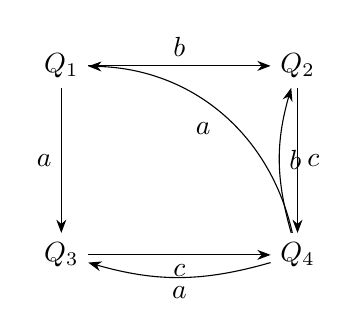
\begin{tikzpicture}[>=Stealth, node distance=2.8cm]
            \node (q1) at (0,1.6) {\(Q_1\)};
            \node (q2) at (3,1.6) {\(Q_2\)};
            \node (q3) at (0,-0.8) {\(Q_3\)};
            \node (q4) at (3,-0.8) {\(Q_4\)};

            \draw[->] (q1) -- node[above] {\(b\)} (q2);
            \draw[->] (q1) -- node[left] {\(a\)} (q3);
            \draw[->] (q2) -- node[right] {\(c\)} (q4);
            \draw[->] (q3) -- node[below] {\(c\)} (q4);
            \draw[->,bend left=16] (q4) to node[right] {\(b\)} (q2);
            \draw[->,bend left=16] (q4) to node[below] {\(a\)} (q3);
            \draw[->,bend right=38] (q4) to node[below left] {\(a\)} (q1);
        \end{tikzpicture}
    \end{center}
    corresponding to
    \begin{align*}
        Q_1 &= b.Q_2+a.Q_3,\\
        Q_2 &= c.Q_4,\\
        Q_3 &= c.Q_4,\\
        Q_4 &= b.Q_2+a.Q_3+a.Q_1.
    \end{align*}

    Starting from the total relation,
    \[
        R_0=\{Q_1,Q_2,Q_3,Q_4\}^2,
    \]
    one application of the functional leaves
    \[
        R_1
        =
        \Id
        \union
        \{(Q_1,Q_4),(Q_4,Q_1),(Q_2,Q_3),(Q_3,Q_2)\}.
    \]
    A second application removes the pairs \((Q_1,Q_4)\) and \((Q_4,Q_1)\):
    \[
        R_2
        =
        \Id
        \union
        \{(Q_2,Q_3),(Q_3,Q_2)\}.
    \]
    The next application is stable, so
    \[
        R_3=R_2=\gfp(F_{\sim}).
    \]

    The same distinction appears in the bisimulation game.
    From \((Q_4,Q_1)\), the attacker can choose the extra transition
    \[
        Q_4\trans{a}Q_1.
    \]
    Matching it with \(Q_1\trans{a}Q_3\) leads to \((Q_1,Q_3)\), where the available actions do not match.
\end{snippetexample}

\pagebreak

\section{Main references}

Useful references include:
\begin{itemize}
    \item K. R. Apt and E.-R. Olderog, \emph{Verification of Sequential and Concurrent Programs};
    \item W. Fokkink, \emph{Introduction to Process Algebra};
    \item R. Milner, \emph{Communication and Concurrency};
    \item A. W. Roscoe, \emph{The Theory and Practice of Concurrency};
    \item H. Bowman and R. Gomez, \emph{Concurrency Theory};
    \item J. C. M. Baeten and W. P. Weijland, \emph{Process Algebra};
    \item M. Hennessy, \emph{Algebraic Theory of Processes};
    \item R. J. van Glabbeek, work on the linear-time--branching-time spectrum;
    \item D. Sangiorgi and D. Walker, \emph{The \(\pi\)-Calculus: A Theory of Mobile Processes}.
\end{itemize}

\end{document}
